%%%%% PREAMBLE %%%%%
\documentclass[11pt,a4paper]{article}
\usepackage{graphicx, float, enumerate} 
\usepackage{amsmath, amssymb, amsfonts} % math stuff
\usepackage{lipsum}
\usepackage[affil-it]{authblk}
\usepackage{setspace}
\usepackage{fancyhdr}
\usepackage{float}
\usepackage{tabularx}
\usepackage{caption}
\usepackage{csquotes} % \enquotes
\usepackage{textcomp}
\usepackage{indentfirst}
\pagestyle{fancy}
\fancyhf{} % Clear default header and footer
\lhead{MODELING INFORMATION DIFFUSION}
\rhead{DERDIYOK}
\usepackage[hidelinks]{hyperref}
\usepackage[sorting=none]{biblatex} % First citation is called 1
\addbibresource{thesis.bib} % Path to your .bib file
\pagenumbering{arabic}
%\parindent 0cm % no paragraph indent
\doublespacing
\begin{document}


%%%%%%%% TITLE %%%%%%%%
\title{Information spread and virality on X (formerly Twitter): a model comparison approach.}
\author{Ekin Derdiyok\\ 
\texttt{\href{mailto:ekin.derdiyok@icloud.com}{ekin.derdiyok@icloud.com}}}
\affil{M.Sc. in Cognitive Neuroscience (MCNB)\\Fachbereich Erziehungswissenschaft und Psychologie
\\Freie Universität Berlin}
\date{\today}
\maketitle
\begin{center}
    \copyright~2024 Ekin Derdiyok    
\end{center}
\pagestyle{plain}



%%%%%%%% ACKNOWLEDGEMENTS %%%%%%%%
\newpage
\doublespacing
\begin{center}
    \section*{Acknowledgements and Author Contributions}     
\end{center}
I would like to express my sincere gratitude to my primary supervisor, Dr. Philipp Lorenz-Spreen, for accepting me as an intern. I am also deeply thankful to Prof. Felix Blankenburg for his interest in the topic and for co-supervising my thesis. A special thanks go to the Max Planck Institute for Human Development for providing me with the opportunity to conduct my internship. I extend my appreciation to Dr. Timo Torsten Schmidt for his guidance and mentorship during the second year. Lastly, I would like to express my gratitude to all the lecturers of the Master Cognitive Neuroscience Berlin (MCNB) program and all the staff at the Department of Education and Psychology at Freie Universität Berlin.

I approached Dr. Philipp Lorenz-Spreen, my primary supervisor, for a master's thesis project towards the end of my internship. I mentioned that I am keen on doing a data modeling project. He suggested several models and journal articles for me to study. Then, we refined the idea together during our first few meetings. This manuscript and the accompanying analysis script were written solely by me. Dr. Philipp Lorenz-Spreen suggested different analyses I can try and commented on the flow of ideas and argumentation in the paper, which I then implemented. This master's thesis is a standalone project and is not part of a greater research project.
 


%%%%%%%% ABSTRACT %%%%%%%%
\newpage 
\begin{center}
    \section*{Abstract}     
\end{center}
The application of network science principles provides a comprehensive understanding of a broad range of complex systems. X (formerly known as Twitter), a popular online microblogging platform, is one such information system where users are connected with follower relationships and information is conveyed between users. In this study, I investigate the diffusion of information by comparing basic mathematical models and compartmental models borrowed from epidemiology to account for the virality claims on Twitter, which is a colloquially shared concept between diseases and social media. Results showed that compartmental models are not especially good at explaining the reach of a tweet, but are open for improvement. The temporal course of a tweet was well captured with a logarithmic function. Models used in this study are compared, and relation to neuroscience research are discussed. \\

Keywords: information diffusion, Twitter, X, network analysis, SIR, social network, Independent Cascade

%%%%%%%% TABLE OF CONTENT %%%%%%%%
\newpage
\tableofcontents

%%%%%%%% INTRODUCTION %%%%%%%%
\newpage
\section{Introduction}
Dynamic systems such as brains, epidemics, social media, or supply chains can be represented as complex networks, wherein they exhibit a similar attribute. In these systems, neural signals, viruses, information, or goods move from one entity to the subsequent one \cite{lewis_network_2011, strogatz_exploring_2001}. Complex networks exhibit an underlying network structure (topology) and flow of interactions or entities (dynamics). Understanding the topology and dynamics of such networks allows scientists of various disciplines to quantify, simulate, predict and therefore better understand a multitude of phenomena \cite{boccaletti_complex_2006}.

Graph theory is the shared go-to method for representing the topology of any such complex network, where a graph is a set of nodes (vertices) and edges (links) \cite{boccaletti_complex_2006}. Having set the topology, dynamics can then be illustrated as the temporal course unfolding as the nodes interact with each other. \hyperlink{sec:network-terms}{Section 1.5 Network terms} repeates and visually demonstrates network science terms.
    
    \subsection{Twitter as a research object}
    Twitter (now known as X), a popular online microblogging platform, can be seen as an amalgam of a social and information network \cite{myers_information_2014, kwak_what_2010}. Henceforth, I will be referring to the platform with the old name Twitter (and not X) to make sure the project is easier to find on search engines and databases. On Twitter, users are socialized either unilaterally (only one user follows the other) or bilaterally (mutual) following. Referring back to complex network nomenclature, for this study, users constitute the nodes; follower relationships define edges. Topology formed by follower relationships allows information to flow between nodes \cite{myers_information_2014}. Possible user interactions enabling information diffusion are tweeting, replying, quoting, liking, and most importantly for the study at hand, retweeting.
    
    Researchers turn to Twitter for a multitude of purposes including sentiment, text, or opinion analyses, as well as investigating information diffusion. A comprehensive systematic literature review of purposes, methods, and metrics used in Twitter research can be found at \cite{firdaniza_information_2021}. According to their literature review, information diffusion proves to be the most prevalent research purpose. Authors have identified a multitude of methods used for studying information diffusion on Twitter. These are epidemic models, Independent Cascade Model, stochastic models, and machine learning. Retweet count was found to be the most prevalent metric used by researchers. The following section exclusively reviews relevant work on information diffusion on Twitter.

    \subsection{Information diffusion on Twitter}
    Previous research has quantified tweet cascades using network science metrics such as depth, size, breadth, speed, structural virality, and clustering to find out how information diffusion differs between groups of tweets with different veracity, content types, or sentiment. Depth indicates the number of layers in the network structure. In Twitter context, this refers to the maximum number of jumps a tweet has to make in order to reach from the source node to the furthest node. Size refers to the total number of nodes or edges in a network graph. In Twitter context, size is the total number of users retweeting a cascade or the total number of follower relationships they have. Breadth of a cascade refers to how many outdegrees a node has. Outdegree refers to the number of directed edges a node has that are starting from the node itself and extending to other nodes. Breadth is usually incorporated as the maximum breadth, that is, the maximum outdegree possessed by any node in the cascade. In Twitter context, maximum breadth refers to the user with the highest follower count. The speed or velocity refers to the inverse of time it takes for a tweet to reach from the source node to the furthest node \cite{juul_comparing_2021}. Clustering refers to the level of connectedness (or the availability of possible edges) within a set of nodes \cite{pierri_topology_2020}. The definition of structural virality metric is murkier. One study defines it as \enquote{the average distance between all pairs of nodes in a diffusion tree [or a cascade, given this paper's nomenclature]}, where distance is referring to the number of jumps an entity has to make in order to reach another node \cite{goel_structural_2016}.
    
    An influential study found that false news spread faster, deeper, and broader than accurate news \cite{vosoughi_spread_2018}, a finding that was then attributed merely to differing cascade sizes and not the veracity of the news per se \cite{juul_comparing_2021}. Pierri et al. has found that underlying network structure differs depending on the veracity of the news shared on social media \cite{pierri_topology_2020}. They were able to label news tweets' veracity by looking at the retweeters' connectedness. For example, participants in a false news cascade were more connected, clustered, and had larger size and depth. This finding is consistent with Vosoughi et al., where it was found that false news are diffusing more strongly on social media on various metrics \cite{vosoughi_spread_2018}. Another study compared virality across different content types (pictures, news, petitions, and videos) and observed that the most viral content type was petition \cite{goel_structural_2016}. Higher virality on petitions can be ascribed to petitions mostly being bottom-up collective causes that citizens come together and push for recognition. This process is clearly dissimilar to broadcast events, such as media outlets sharing news articles or celebrities sharing images. Emotional tweets tend to differ from factual tweets. Antypas et al. found that negative sentiment in politicians' tweets contributes to a higher retweet count \cite{antypas_negativity_2023}. Likewise, Meng et al. found that perceived negative emotion, but not positive, predicted both diffusion size and structural virality \cite{meng_diffusion_2018}. They also found that perceived efficacy about health-related issues was positively correlated with diffusion size. In short, many attempts have been made to understand the factors contributing to humans' information sharing behavior.
    
    \subsection{Modeling information diffusion}
    Several attempts have been made to model information diffusion on Twitter using various models, both off-the-shelf and custom-built. One such study used the Susceptible-Infectious-Recovered (SIR) model to investigate factors contributing to a tweet's spread \cite{zheng_factors_2018}. Authors found that the content of a message holds more influence than the popularity of the sender. SIR model is a compartmental model, that is, it divides entities (e.g., users) into compartments (i.e., states) to account for the flow of entities between these compartments (i.e., state transition) \cite{kermack_contribution_1927}.
    
    Muhlmeyer et al. had a very similar approach to the current study by modeling information diffusion using compartmental models \cite{muhlmeyer_modeling_2020}. They proposed compartmental models that are variants of conventional SIR model with increasing complexity and more realistic assumptions that would fit into an information diffusion context. The most basic version they suggest is the Ignorant-Spreader (IS) model, where Ignorant corresponds to information-naive users and Spreader who “infect” Ignorant. The Ignorant-Spreader-Recovered (ISR) model is one-step more complex, which accounts for Spreaders ceding to be Spreaders by “recovering”. They go further to suggest a social media variant of the model, which accounts for the decaying attention on a topic.
    
    Apart from SIR and its variants, the Independent Cascade (IC) model has also been utilized by researchers to study information diffusion. The IC model is another compartmental model that is more common in information, technology adoption, and marketing as opposed to the SIR model, which has its roots in epidemiology. Put simply, the IC model is an extension of the SIR model with an extra constraint, that is, each node has a single chance at infecting its neighbors. In other words, if a node fails to infect one of its neighbors in any given trial, the connection between them is ineffective for the rest of the trials \cite{kempe_maximizing_2003}. One study used the IC model in the context of influence maximization \cite{kim_study_2015}. Although the IC model is of great interest for this paper, details of this particular study are not discussed, as influence maximization is a distinct field of research from information diffusion.
    
    \subsection{Temporal patterns of information diffusion}
    The aforementioned models use discrete time steps to model the spread of a tweet cascade. Both SIR and IC models have a parameter for number of iterations, which is an abstracted time unit, ignoring the time as we understand (i.e., hours passed). Another approach to analyze a tweet cascade is to make use of the time and is a tweet's evolution over time. Zhao et al., propose a model to predict the popularity of a tweet by incorporating \textit{infectiousness} and \textit{time passed} parameters into their model. Their model offers significant improvements over simpler baseline models in predicting retweet count at any given time point within a cascade's evolution \cite{zhao_seismic_2015}. Stai et al. suggest a model to capture decreasing infectiousness over time (due to Twitter timeline algorithm or any other cause) and compare how tweets of different topics behave (defined as a hashtag) \cite{stai_temporal_2018}. They found that, over time, some more general topics have a relatively stable infectiousness rate (e.g., \#2014moments, \#springbreak), whereas event-specific topics are better modeled with a varying infectiousness parameter.

    \subsection{Network terms}
    \hypertarget{sec:network-terms}{}
    It is essential to map the network terms, as not all studies treat the same constructs as nodes or edges. The graph refers to the topology of users and the follower connections (or lack thereof) for each cascade. It is represented as a matrix of users, where row and column labels are different nodes and values are the edges. Graphs in this study are binary (i.e., unweighted) and directed (i.e., unilateral connection). \hyperlink{fig:figure1}{Figure 1} and \hyperlink{fig:table1}{Table 1} show which term maps to which empirical construct. In the current study, nodes are Twitter users. Not all Twitter users are modeled as a node in this study. The complete set of nodes corresponds to the combination of follower networks of each user who participated in a given tweet cascade. Edges refer to directed follower relationships. Two users may bilaterally follow each other, or there may be a unilateral relationship where a user follows the other user. A tweet cascade is a chain of tweets extending the source tweet via retweets. All the tweets in a tweet cascade are effectively the copies of the original tweet. This study employs multiple tweet cascades, where each one will be modeled independently, meaning that as many models were fit as there are cascades. This study exclusively investigates tweeting (original posts) and retweeting (copies of the original posts), without differentiating comments and quotes.\\
    
\begin{figure}[H]
    \hypertarget{fig:figure1}{}
    \centering
    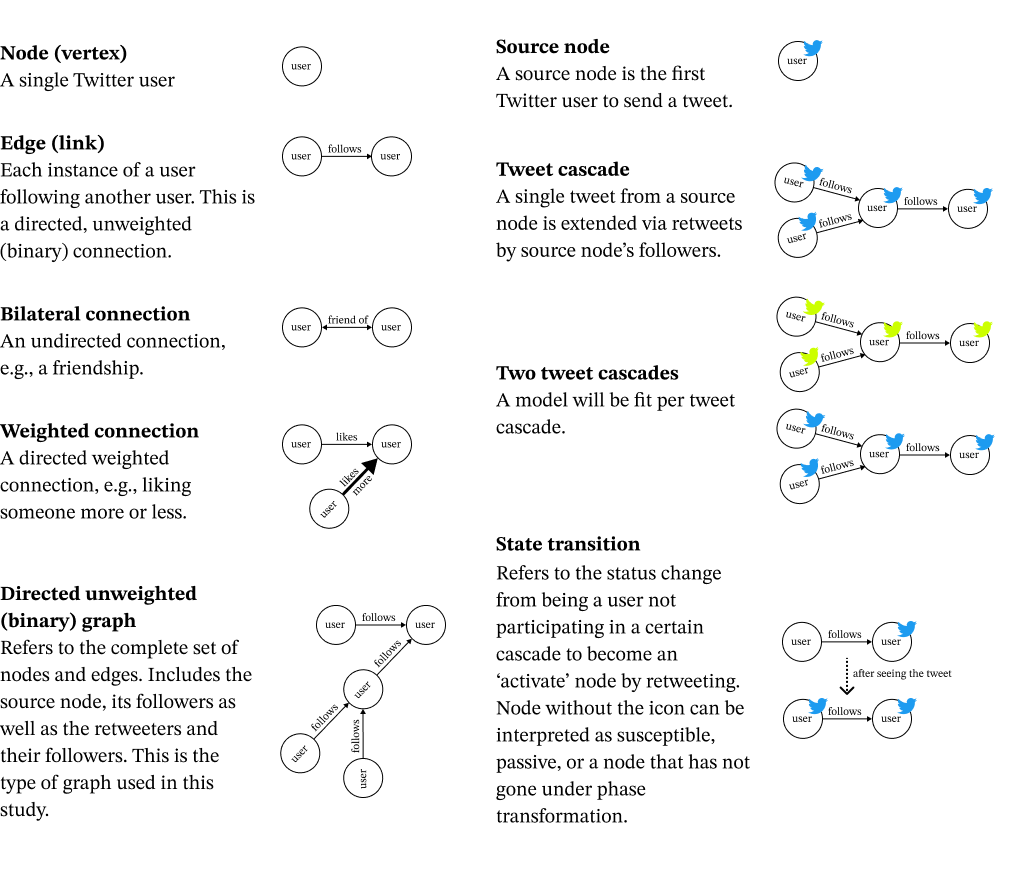
\includegraphics[width=1\linewidth]{thesis_network_terms.png}\\
    \caption{Network science terms and how they are mapped to empirical constructs in the current study.}        
    \label{fig:enter-label}
\end{figure}

\begin{table}[h]
    \hypertarget{fig:table1}{}
    \label{tab:table1}
    \centering
    \small
    \begin{tabularx}{\textwidth}{|l|X|}
        \hline
        \textbf{Term} & \textbf{Explanation} \\
        \hline
        Information diffusion & Spread or dissemination of information via retweets  \\
        Tweet & A single unit of a short post on Twitter \\
        Retweet & Copies of a tweet, usually made by other users on Twitter \\
        Retweet count & Number of times a tweet was retweeted \\
        User & Any Twitter account owner that is part of the study \\
        Follower & A user who follows another user, i.e., is likely to another user's tweets \\
        Followee & A user who is being followed by a follower \\
        Cascade & Set of a single unique tweet and its retweets \\
        Topology & Follower network structure of a user or a cascade \\
        Dynamics & Information diffusion on a given topology \\
        Viral & An information diffusion characteristic defined by the large sum of smaller user-to-user interactions \\
        Broadcast & An information diffusion characteristic referring to cascades initiated by a mass communication medium (e.g., celebrities, news outlets, politicians) \\
        Semantic category & Whether a tweet is factual or emotional/personal \\
        Topic & Specific subject of the tweet \\
        Mean-field model & A kind of model that approximates interactions between agents as averages \\
        Network model & A more specific kind of model that accounts for the topology \\
        Compartmental & Set of models that divides agents into different subgroups and examines the flow between subgroups \\
        Infectiousness  & Likelihood of a tweet being retweeted, $\beta$, $p_{uv}$ \\
        Feed & Continuously updating stream of tweets \\
        NLP & AI subfield striving to enable computers understand human language \\
        LLM & AI models striving to understand and generate human language \\
        State & Specific condition of a node, e.g., susceptible or infected \\
        State transition & Any changes between conditions, e.g., moving from susceptible to infected \\
        \hline
    \end{tabularx}
    \caption{Terminology used in this study.}
\end{table}
    
    \subsection{Aim of the current study}
    The aim of this study is threefold: modeling information diffusion on Twitter using compartmental models. By increasing model complexity gradually, I strive to find out which parameters and assumptions ensure a greater model fit. Then, identifying the effects of message content on message dissemination. Finally, investigating time series behavior of cascades. Hypotheses are not specified due to the predominantly exploratory nature of the study. Yet, research questions are laid out formally in the following section.

    \subsection{Research questions}
        \begin{enumerate}
            \item[RQ1:] Which model assumptions and parameters will capture cascades' retweet counts best?
            
            \item[RQ2:] How to best describe the temporal properties of a cascade's diffusion?
            
            \item[RQ3:] Do tweets with different topics or semantic categories (i.e., whether a tweet is emotional/personal or factual) have different model parameters?
        \end{enumerate}

%%%%%%%% METHODS %%%%%%%%
\clearpage
\section{Methods}
    \subsection{Data and code availability}
    Data feature English-language tweets from 2015 Nepal earthquake between 2015-04-25 and 2015-04-27. It is downloaded from a open-access online repository \cite{bhowmick_twitter_2019}. No ethics approval were issued for the study at hand. Although the initial idea was to fetch data from Twitter API, this plan had to be abandoned due to unforeseen changes in the Twitter API pricing plan, which is discussed in greater detail in the discussion section. The analysis script along with data are stored on an online repository and is publicly available on \href{https://github.com/ekinderdiyok/information-diffusion-on-twitter}{https://github.com/ekinderdiyok/information-diffusion-on-twitter}. The analyses can be reproduced by installing the necessary packages (notice the packages imported in the code) downloading both the data and analysis, placing data files in the same folder and entering the file path to the relevant field in the analysis script. Data files in the repository branch out from the what is publicly available on Zenodo \cite{bhowmick_twitter_2019}. My repository includes an extra file \texttt{(cascades.csv)} which has information on topic and semantic category of each tweet (more on this in \hyperlink{sec:tagging-tweet-topic}{Section 2.5 Tagging tweet topics and sematic categories}), as well as total retweet count and full text of each cascade. These information had to be saved because the former two costs OpenAI credits, and the latter two was manual labor (not reproducible by code).

    \subsection{Materials}
    The analyses were run on Jupyter Notebooks (6.4.12) running Python (3.9.13 (main, Aug 25 2022, 18:24:45) [Clang 12.0.0 ]), distributed by Anaconda Distribution, Anaconda\textregistered. OpenAI API was used to create major topics and clustering tweets into these topic \cite{openai_llc_openai_2023-1}. NDlib was used for basic diffusion models \cite{rossetti_ndlib_2018,rossetti_ndlib_2017}. NetworkX was used for creating network topology \cite{hagberg_exploring_2008}.
    
    \subsection{Procedure}
    Data were downloaded, imported, preprocessed, and analysed locally on my personal computer. Full text information and the number of current followers were absent in the dataset. These data had to be manually collected by browsing tweet IDs on a web browser. For example, the following URL will lead to the tweet with tweet id \texttt{1648416432223404033} \href{https://twitter.com/anyuser/status/1648416432223404033}{https://twitter.com/anyuser/status/1648416432223404033}.
    
    Parameter estimation was done by using \texttt{scipy.optimize.minimize\_scalar} function from SciPy library \cite{virtanen_scipy_2020}. This function was used to return the value that minimizes mean absolute deviation between model simulations and observed retweet counts. Absolute deviations were calculated for all cascades. Then, it was summed and passed into the \texttt{scipy.optimize.minimize\_scalar} function. This function returned the minimizer value, that is, the parameter estimate, that returns the lowest mean absolute deviation for the given model. Minimizer was then interpreted as the fitted model parameter.
    
    After estimating the best fitting model parameters. Simulations were run to evaluate each of the model by calculating the explained variance $R^2$ and mean absolute deviation ($MAD$). Mean absolute deviation was preferred over mean sum of squares, since this dataset is rich in outliers and mean sum of squares penalizes larger deviations more than smaller deviation, making the outliers even more influential in models. The network structure for each cascade were constructed from follower relationships. The following section describes how network graphs were constructed.

    \subsection{Network graphs}
        Network graphs in this study are based on follower relationships. Directed (unilateral) follower connections between nodes were mapped. Direction of edges are from the followee (user who is being followed) node to the follower node. In other words, it mimics the direction of information flow. For each cascade, a separate network graph was constructed. First, the source node and retweeters were added as nodes to the graph. Then, all the followers of these nodes were also added with directed edges in between.
        
        \hyperlink{fig:network}{Figure 2} illustrates the social network structure of cascades by plotting them as network graphs. Network models (SI and IC) are based on the these network graphs. \hyperlink{fig:network}{Figure 2} should help readers better understand the network models used in this project. Top-left cascade demonstrates comparable contribution from multiple users, top-right cascade demonstrates a less influential source nodes, being supported by several well-connected nodes. Bottom figures feature two tweet cascades without the black nodes (i.e., followers of retweeters who has not retweeted). This figure should illustrate what how an actual tweet cascade looks like in the current study.

        \begin{figure}[H]
            \hypertarget{fig:network}{}
            \centering
            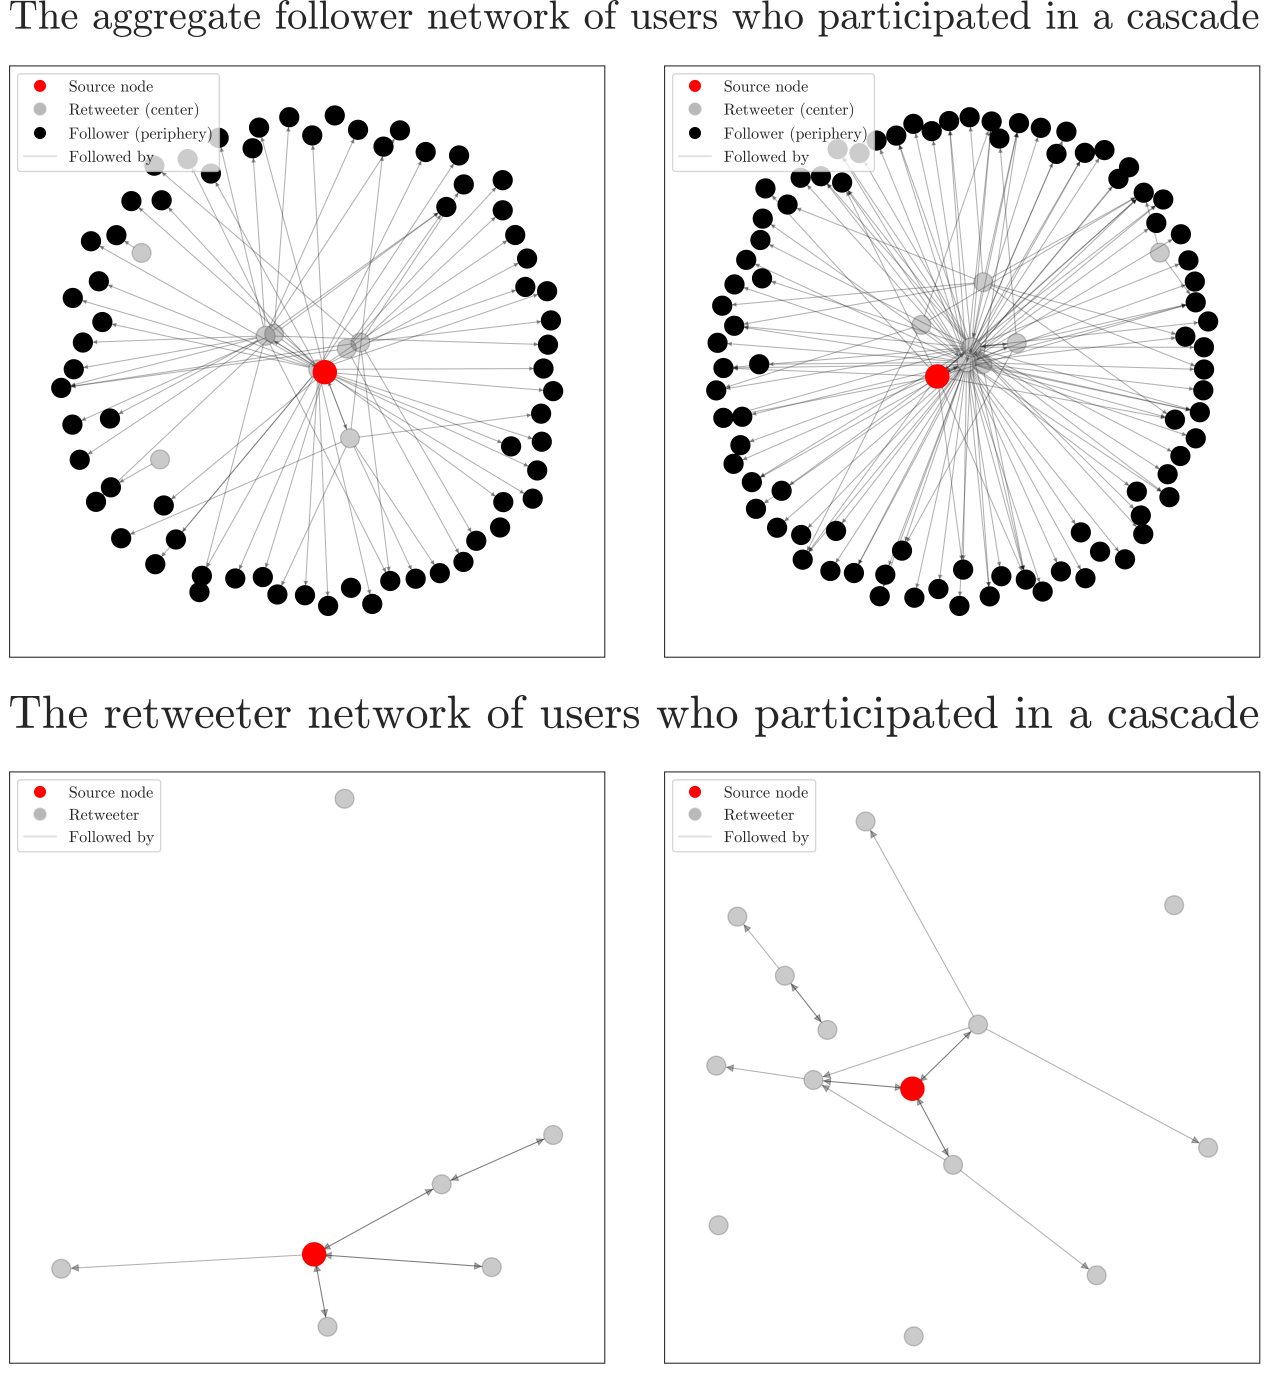
\includegraphics[width=1\linewidth]{thesis/retweeter_network_post.png}\\
            \caption{Network graphs of four cascades shown in spring layout. Top two graphs are featuring the source node, retweeters, and followers. Bottom two excludes followers to better visualize the retweet cascade structure. [red node] Source node, i.e., original poster of the tweet. [grey nodes around center] Users who retweeted the tweet. [arrows] Follower relationships, read as \enquote{node A followed by node B} following the direction. [black nodes in periphery] aggregate follower network of the source node and all retweeters, who has not retweeted the tweet. [standalone grey dots] Retweeted the cascade but has no follower relationship with any other retweeter. Note: On the top two graphs, only 3\% of the followers (black nodes) were plotted to overcome overplotting.}    
            \label{fig:enter-label}
        \end{figure}
    
    \subsection{Tagging tweet topics and semantic categories}
    \hypertarget{sec:tagging-tweet-topic}{}
    Topic clusters were identified using OpenAI's GPT-3.5, a large language model (LLM)\cite{openai_llc_openai_2023}. This approach was inspired by Rathje et al., as a quick yet accurate substitute for natural language processing (NLP) \cite{rathje_gpt_2023}. Since the whole dataset exceeded the token limitation of the model, large chunks of tweets were inputted to the model with the following prompt: 

    \begin{quote}
         \texttt{The following is a large collection of tweets about the Nepal 2015 earthquake. Identify major  topic clusters: [here goes ~50 tweets separated by paragraphs]}   
    \end{quote}{}

    
    After having identified the topic clusters, duplicates and semantically overlapping topics emerged, due to independently prompting the model several times. These were manually merged by the author. For example \textit{relief efforts and resources}, \textit{relief efforts and assistance}, \textit{donations and relief efforts}, \textit{charitable donations and fundraising}, and \textit{Infrastructure and resources} were merged under the topic name \textit{relief efforts, resources, donations, and infrastructure}.
    
    As a last step, tweets were categorized into topics using OpenAI API official Python bindings \cite{openai_llc_openai_2023}. The model was prompted once for each tweet, asking which of the following topic best describes the tweet at hand. The following prompt was used:
    \begin{quote}
        \texttt{Only write the name of the topic which fits the following tweet best. Choose one of the following possible answers: \\
        1. Rescue operations and assistance \\
        2. Impact, aftermath, death toll \\
        3. Aftershocks and tremors \\
        4. International response and international support \\
        5. Technology, communication, and social media \\
        6. Controversy, criticism, social and political commentary \\
        7. Relief efforts, resources, donations, and infrastructure \\
        8. Faith and prayers \\
        9. Personal experience, stories, and missing people \\
        10. The tweet does not fit any of the given topics. \\
        Following text is the tweet: [here goes a single tweet]} 
    \end{quote}

    
    To come up with an inter-rater reliability measure, resulting topics were then compared with a human tagging the topics (author himself). Cohen's Kappa  indicated a substantial, but not perfect, agreement between the human and machine topic tagging $(\kappa = .64)$ \cite{cohen_coefficient_1960}. A similar approach was pursued for marking tweets' semantic category, that is, whether they are emotional/personal or factual $(\kappa = .71)$.

    \subsection{Models used in this study}
        \subsubsection{Null model}
        A simple linear regression has predicted retweet counts based solely on follower count. Linear regression served as a null model (i.e., a benchmark) against which subsequent models could be compared. The model was studied to be extended further (into a multiple linear regression) by incorporating other tweet characteristics such as, message length and emotionality.

        \begin{equation}
            f(x) = ax + b
        \end{equation}
        
        \subsubsection{Mean-field Susceptible-Infectious model}
        The mean-field version of the Susceptible-Infectious (SI) model from epidemiology was employed \cite{downey_epidemiology_2022}. The SI model, traditionally used to simulate disease spreads, was adapted to characterize the information diffusion within the context of retweeting behavior. Mean-field SI model can be formalized as a pair of differential equations \hyperlink{eq:eq1}{(Equations 2 and 3)}. $s$ represents the susceptible population (followers of a user), $i$ represents the number of infected individuals (retweet count). $\beta$ represents the infectiousness. In Twitter context, it refers to how likely a follower is to retweet a tweet. $\dfrac{ds}{dt}$ and $\dfrac{di}{dt}$ represents the rate of state transition in susceptible and infected individuals over time, respectively. The model starts with only one infected node, that is the source node ($i = 1$). Number of susceptible individuals are equal to the number of followers ($s = n_{followers}$). The diffusion process iterates in discrete time steps. In the first step, there is only one infected node. The choice of number of steps is at the modeler's discretion. In this study, all models were iterated four times, including the first step where, by definition, only one node is infected. This is equivalent of a user seeing a tweet on their feed for three times.

        \begin{equation}
            \hypertarget{eq:eq1}{}
            \frac{ds}{dt} = -\beta s i
        \end{equation}
    
        \begin{equation}
            \frac{di}{dt} = \beta s i
        \end{equation}

        \subsubsection{Network-based Susceptible-Infectious model}
        A network version of the SI model was used to model the retweet count of each cascade \hyperlink{eq:network-SI}{(Equations 4 and 5)} \cite{kermack_contribution_1927}. 

        $\dfrac{dS(t)}{dt}$ stands for the rate of chance of number of susceptible individuals in time $t$. $\dfrac{dI(t)}{dt}$ does the same for infected individuals. $N$ stands for the total number of users affiliated with a cascade, that is, the total count of source node, retweeters, and their followers. By definition $N = S + I$ at any time point $t$. $A_{ij}$ is the adjacency matrix where $i$ corresponds to the row index and $j$ corresponds to nodes the column index. $A_{ij}$ takes the value $1$ only when node $i$ follows node $j$ and $0$ if this condition is not satisfied. $A_{ij} I_j(t)$ maps the edges between each infected node and their followers.
            
        In the SI model, the diffusion process unfolds in discrete time steps as well. As opposed to mean-field SI model, each node has a certain chance of influencing only its neighbors, hence making them infected. In the network variant of the model, nodes can only affect their neighboring nodes, as opposed to the mean-field version where all nodes, regardless of their topology, affect each other. The network version of the SI model comes with the benefit that it takes into account how well each node is connected. Put differently, nodes with higher follower count are more influential in the sense that they can potentially infect a larger number of susceptible users. Like described above, the model starts with a single infected source node (the original poster of the cascade). In the SI model, number of susceptible individuals equal to the node count in the aggregate follower network of all retweeters (i.e., cascade participants). In other words, network graphs of the source node and retweeters are combined to define the susceptible population.

        \begin{equation}
            \hypertarget{eq:network-SI}{}
            \frac{dS(t)}{dt} = - \beta \sum_{i=1}^N \sum_{j=1}^N A_{ij} I_j(t) 
        \end{equation}

        \begin{equation}
            \frac{dI(t)}{dt} = \beta \sum_{i=1}^N \sum_{j=1}^N A_{ij} I_j(t)
        \end{equation}



        A drawback of the SI model is that it assumes that infected nodes (nodes that have gone under state transition and are now in the “I” compartment) stay infected forever. Meaning that they can influence all of their neighboring nodes over all the model iterations. In other words, each node has a chance to infect all of its neighboring nodes over the whole life-cycle of a tweet cascade. This, however, is an unrealistic assumption for Twitter. Because, unlike an epidemic, Twitter users come across a tweet only a few times before it is buried down in their feeds.

        \subsubsection{Independent Cascades model}
        The Independent Cascades (IC) model addresses the aforementioned drawback of SI model. The IC model was employed to account for the one-time exposure to a copy of a tweet on a user's timeline. In the IC model, each node has only one chance to activate each of its neighboring nodes \cite{kempe_maximizing_2003}. Put differently, if a node is infected on a given iteration, it has only one shot (on the next iteration) infecting its neighboring nodes. If infection does not happen, given node is effectively \enquote{recovered} and cannot infect.
        
        Suppose user $U_1$ retweeted a certain tweet on second iteration of the model, $U_1$ can make her neighbors (let neighbors be $U_2$ and $U_3$) retweet during the third iteration. If neither $U_2$ nor $U_3$ retweets the cascade on third iteration, $U_1$ does not hold a chance on the fourth iteration. Still, $U_4$ (let $U_4$ be a node that got infected on third iteration and is a neighbor of $U_2$ and $U_3$) can infect $U_2$ and $U_3$.    
        
        \hyperlink{eq:IC}{Equation 6} explains the IC model with its mathematical equation. $P_v(t)$ represents the probability of node $v$ to go under state transition at time step $t$. $p_{uv}$ models the probability of node $u$ to causing a state transition at node $v$. $1-p_{uv}$ represents the complementary event, i.e., probability of node $u$ to fail to cause a state transition at node $v$. $\prod_{u \in N(v)} (1 - p_{uv})$ represents the combined probability of all neighboring nodes $u$ failing to cause a state transition at node $v$.
        
        \begin{equation}
            \hypertarget{eq:IC}{}
            P_v(t) = 1 - \prod_{u \in N(v)} (1 - p_{uv})
        \end{equation}

        \subsubsection{Decaying IC model}
        All the models listed so far have a fixed infectiousness or threshold parameter ($\beta$ or $p_{uv}$) for determining whether an infection will happen on a given round. On Twitter, however, recent posts are favored over older posts by the feed algorithm and most cascades are shallow due to the attention and interest of users' being dispersed \cite{lorenz-spreen_accelerating_2019, twitter_inc_twitters_2023}. Furthermore, the likelihood of a retweet chain, that is, a retweet being retweeted, is low \cite{goel_note_2015}. Concisely, as time passes infectiousness of a tweet decreases.
        
        To make the model capture Twitter's reality better, I created a custom version of the IC model where the infectiousness parameter goes under an exponential decay (\hyperlink{eq:decay}{Equation 7}) where $\lambda$ (lambda) is the decay constant, with higher values corresponding to a faster decay. $p_{uv}$ is the initial infectiousness. As the diffusion process unfolds over many iterations, infectiousness parameter exponentially decays to become smaller and smaller.

        \begin{equation}
            \hypertarget{eq:decay}{}
            p_{uv}(t) = p_{uv} \cdot e^{-\lambda t}
        \end{equation}

        Hence, the decaying variant of the IC model is:

        \begin{equation}
            \hypertarget{eq:dec-IC}{}
            P_v(t) = 1 - \prod_{u \in N(v)} (1 - p_{uv} \cdot e^{-\lambda t})
        \end{equation}

        \hyperlink{eq:dec-IC}{Equation 8} replaces the term $p_{uv}$ in \hyperlink{eq:IC}{Equation 6} with $p_{uv} \cdot e^{-\lambda t}$.

        \subsubsection{Empirical cumulative distribution function}
        Until now, for all the models above, temporal course was represented as discrete steps or iterations. To get a better picture of temporal properties of information diffusion on Twitter, empirical cumulative distribution functions (ECDFs) were used. ECDF provides insights into the temporal distribution of retweets. First, timestamps of all retweets of a cascade are ordered to ascend. Then, the cumulative proportion of timestamps that are below the given timestamp are calculated. ECDF values are interpreted similar to quantiles, such that ECDF function takes values between 0 (the first timestamp, which has no timestamps preceding it) and 1 (the last timestamps, which is larger than all the other timestamps) \cite{conover_practical_1999}. 
        
        For example, in the context of this study, a timestamp having an ECDF value of 0.69 means that 69\% of all timestamps in cascade have a value that is equal to lower than the given timestamp. Put differently, 69\% of all the retweets the given cascade will receive are before the given timestamp. 
        
        \hyperlink{eq:ECDF}{Equation 9} shows the formal definition of ECDF, where $F(x)$ is the ECDF value, $I(x_i \leq x)$ is an indicator function returning 1 if the condition is met, 0 if not. $x_i$ is the individual data points. $\sum_{i=1}^{n} I(x_i \leq x)$ counts the number of $x_i$'s that are below $x$.  $\dfrac{1}{n}$ ensures that the ECDF value $F(x)$ stays between 0 and 1.

        \begin{equation}
            \hypertarget{eq:ECDF}{}
            F(x) = \frac{1}{n} \sum_{i=1}^{n} I(x_i \leq x)
        \end{equation}

        \subsubsection{Sigmoid function and Avrami equation}
        \hypertarget{sec:sigmoid}{}
        The shape of the empirical cumulative distribution was compared with a sigmoid function. Sigmoid function is hypothesized to capture the distinct phases of viral-like diffusion behavior of tweets (\hyperlink{fig:sigmoid}{Figure 3}). Namely, (1) the initial phase, representing the initial viral diffusion of information. In this phase, growth has started slow but is exponential. (2) Accelerated growth stage, which is characterized by the fastest growth. (3) Slowing growth stage, wherein a retweet gradually loses traction as users shift their interests or the feed algorithm favoring more recent posts to the one at hand. And finally (4) saturation stage, where most the cascade has seen most of its growth.
        
        \begin{figure}[H]
            \hypertarget{fig:sigmoid}{}
            \centering
            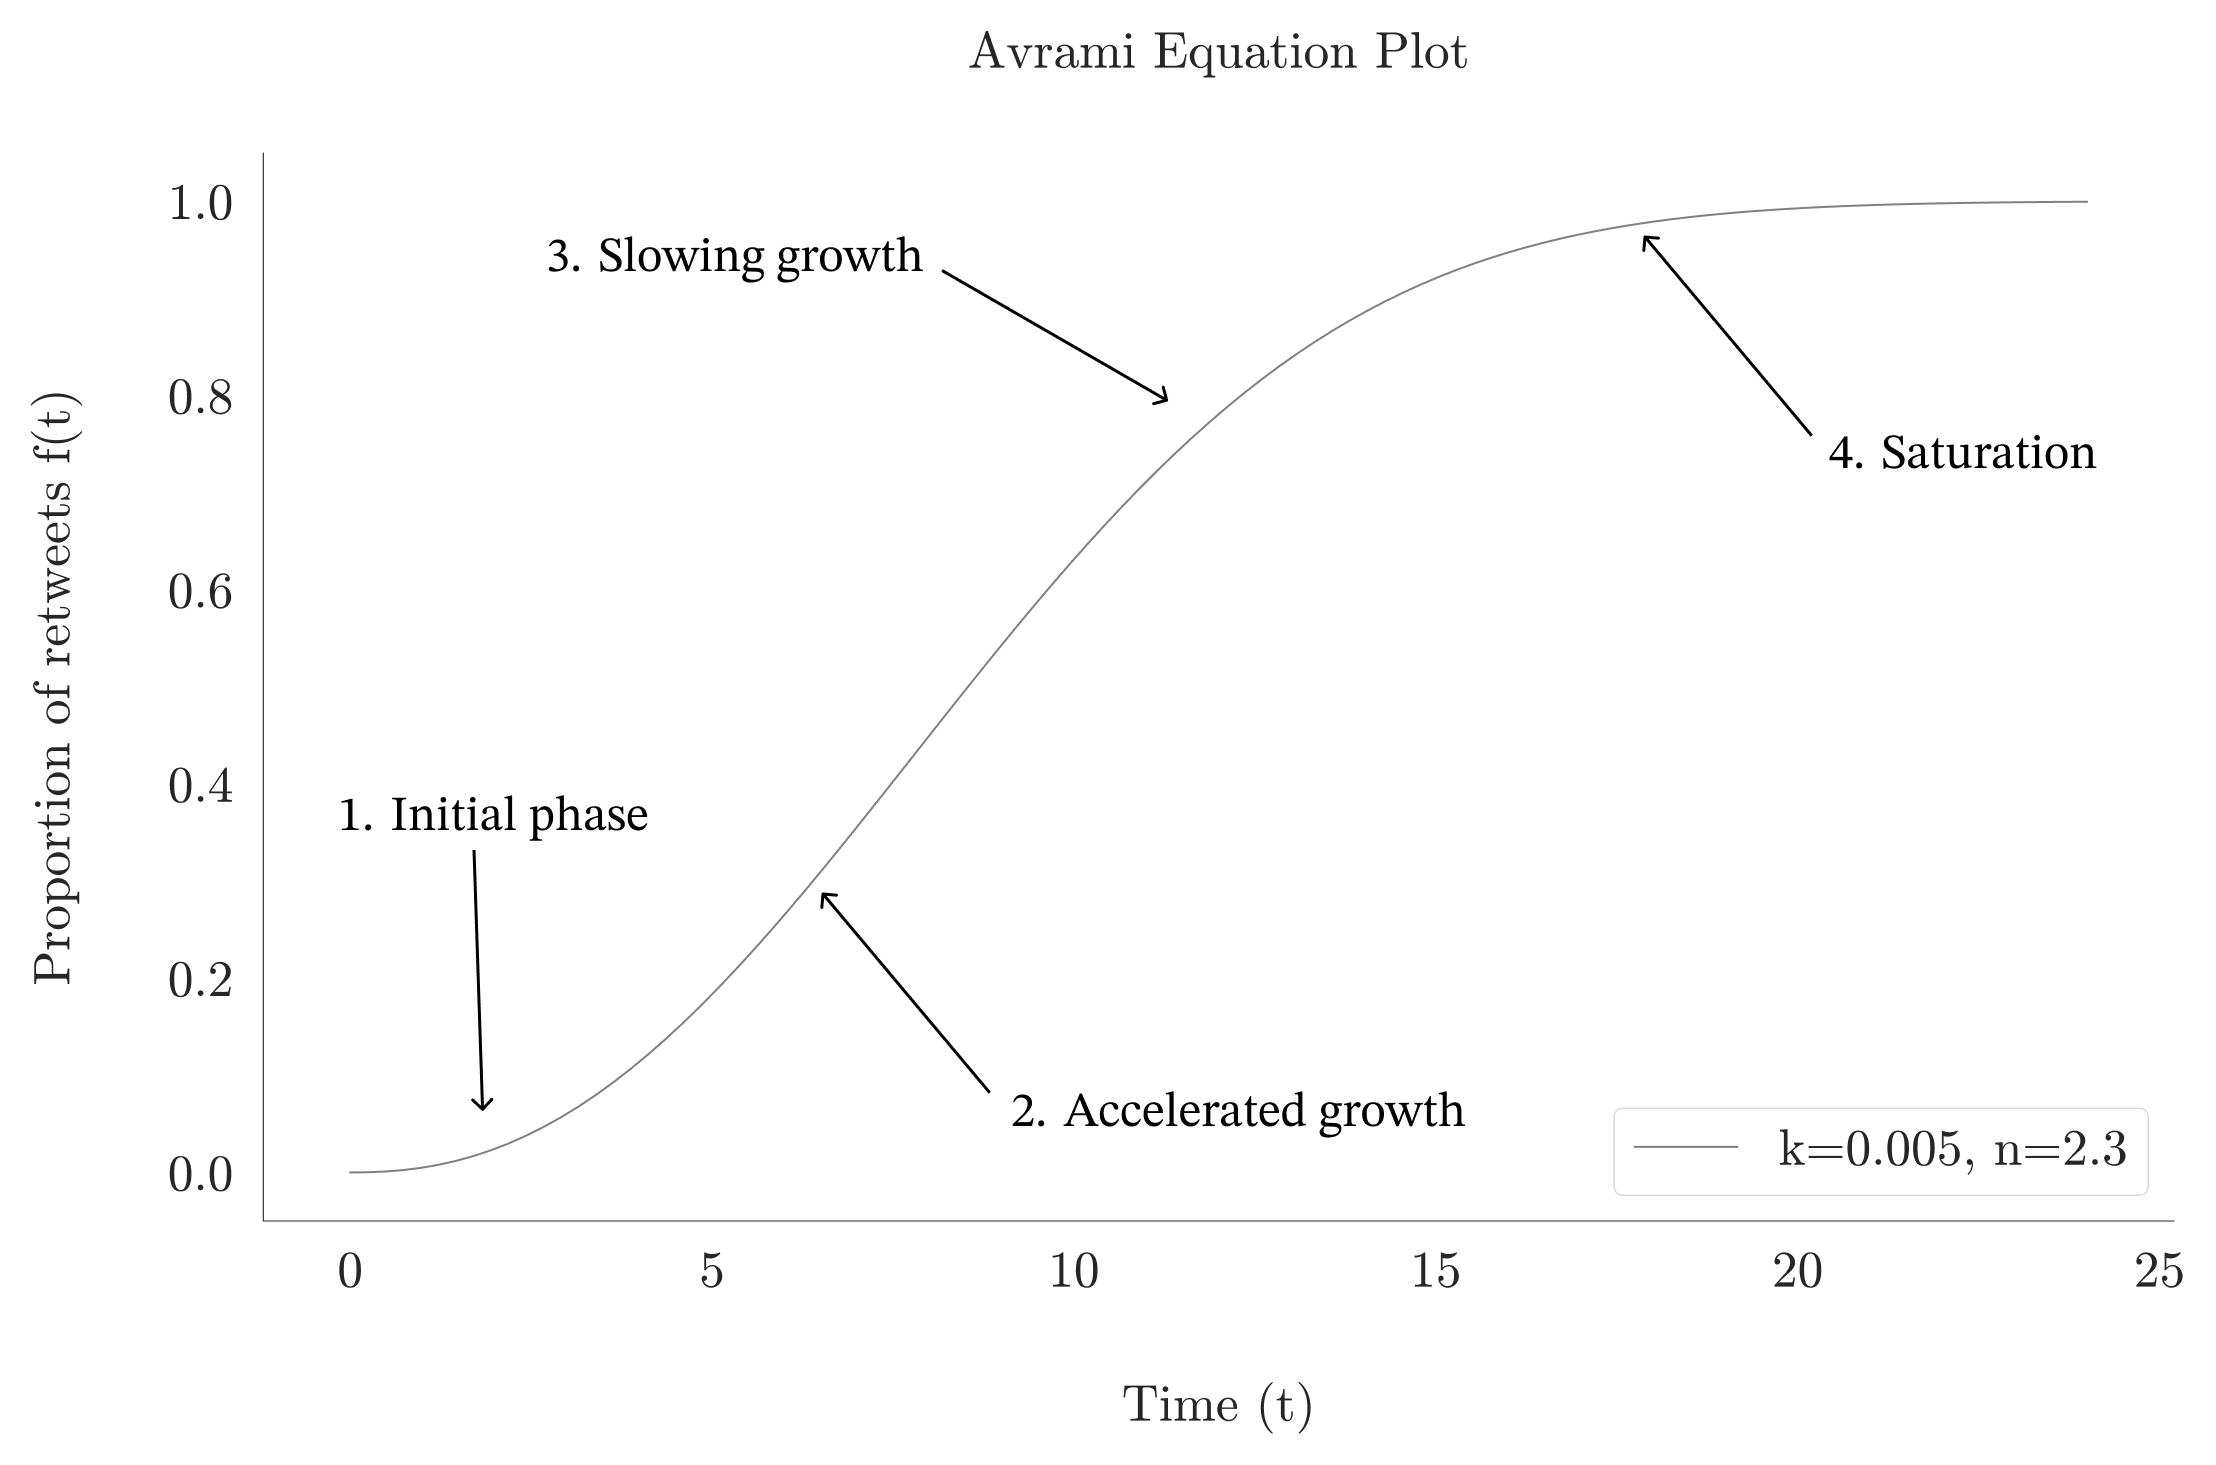
\includegraphics[width=1\linewidth]{thesis/avrami_post.png}\\
            \caption{ECDF plot of shape sigmoid function, formalized by an Avrami equation. Figure 3 demonstrates why sigmoid function is hypothesized to be a good fit for the temporal course of a cascade. Arguments $k = 0.005$, $n = 2.3$, $t_{max} = 24$ were picked arbitrarily to show four distinct states clearly.}
            \label{fig:enter-label}
        \end{figure}
        
        Sigmoid function in this study is expressed with the Avrami equation (\hyperlink{eq:avrami}{Equation 10}). Previous literature  has utilized Avrami equation \cite{shirzad_critical_2023}, for explaining time series behavior of viral diffusion \cite{avramov_kinetics_2007}, citation networks \cite{sangwal_comparison_2021}, and spread of religions \cite{ausloos_statistical_2007}. Here, the same idea is applied to information cascades.

        \begin{equation}
            \hypertarget{eq:avrami}{}
            f(t) = 1 - \exp\left(-k \cdot t^n\right)
        \end{equation}

        In the context of this study, $f(t)$ represent the proportion of retweets in a cascade that has been sent. It is a measure of the life-cycle of the cascade at time $t$. $k$ is the rate constant, which symbolizes the infectiousness of a tweet.  $t$ is the time. $n$ represents the dimensionality of the spread of the disease. For example, $n=1$ would represent a linear information diffusion where diffusion unfolds in a line. $n=2$ would represent a two dimensional spread where the information diffusion can become exponential. $n=3$ would potentially represent a more complex and elaborate diffusion pattern. Discussion of the $n$ parameter and what it would specifically mean in information diffusion or epidemiology is beyond the scope of this study.

        \subsubsection{Logarithm function}
        An argument can be made for why a logarithm function can be a better fit than the sigmoid function for temporal evolution of Twitter cascades. Twitter algorithm favors recent posts over older posts \cite{twitter_inc_twitters_2023} and users lose attention in a topic fairly quickly \cite{lorenz-spreen_accelerating_2019}.
        
        Best fitting $a$ and $b$ parameters will be estimated by fitting a logarithm function to the empirical cumulative distributions of all cascades (\hyperlink{eq:log}{Equation 11}). Logarithm function is expected to reflect the initial burst of retweets in the first few hours of a tweet, followed by a slower, sustained information diffusion thereafter.

        \begin{equation}
            \hypertarget{eq:log}{}
            f(t) = a \cdot log_{10}(t) + b
        \end{equation}

        Where $f(t)$ is the ECDF value, i.e., proportion of retweets that are sent by the the given time $t$.

%%%%%%%% RESULTS %%%%%%%%
\clearpage
\section{Results}

    \subsection{RQ1}
    Retweet count was investigated with four models starting with a simple linear regression and building up complexity each time to assess their efficacy in predicting retweet counts and whether they are outperforming its predecessor.
        
    Simple linear regression showed that follower count was a weak predictor of retweet count, $R^2 = .13$, 
    $Mean \, Absolute \, Deviation \ (MAD) = 31.16$ \hyperlink{fig:null-model}{Figure 4} shows a scatter plot with a linear regression fit, where each point corresponds to the follower count of original poster (x-axis), and the retweet count (y-axis). The plot is in log-scale to account for the retweet counts and follower counts that differ in orders of magnitude.

    \begin{figure}[H]
        \hypertarget{fig:null-model}{}
        \centering
        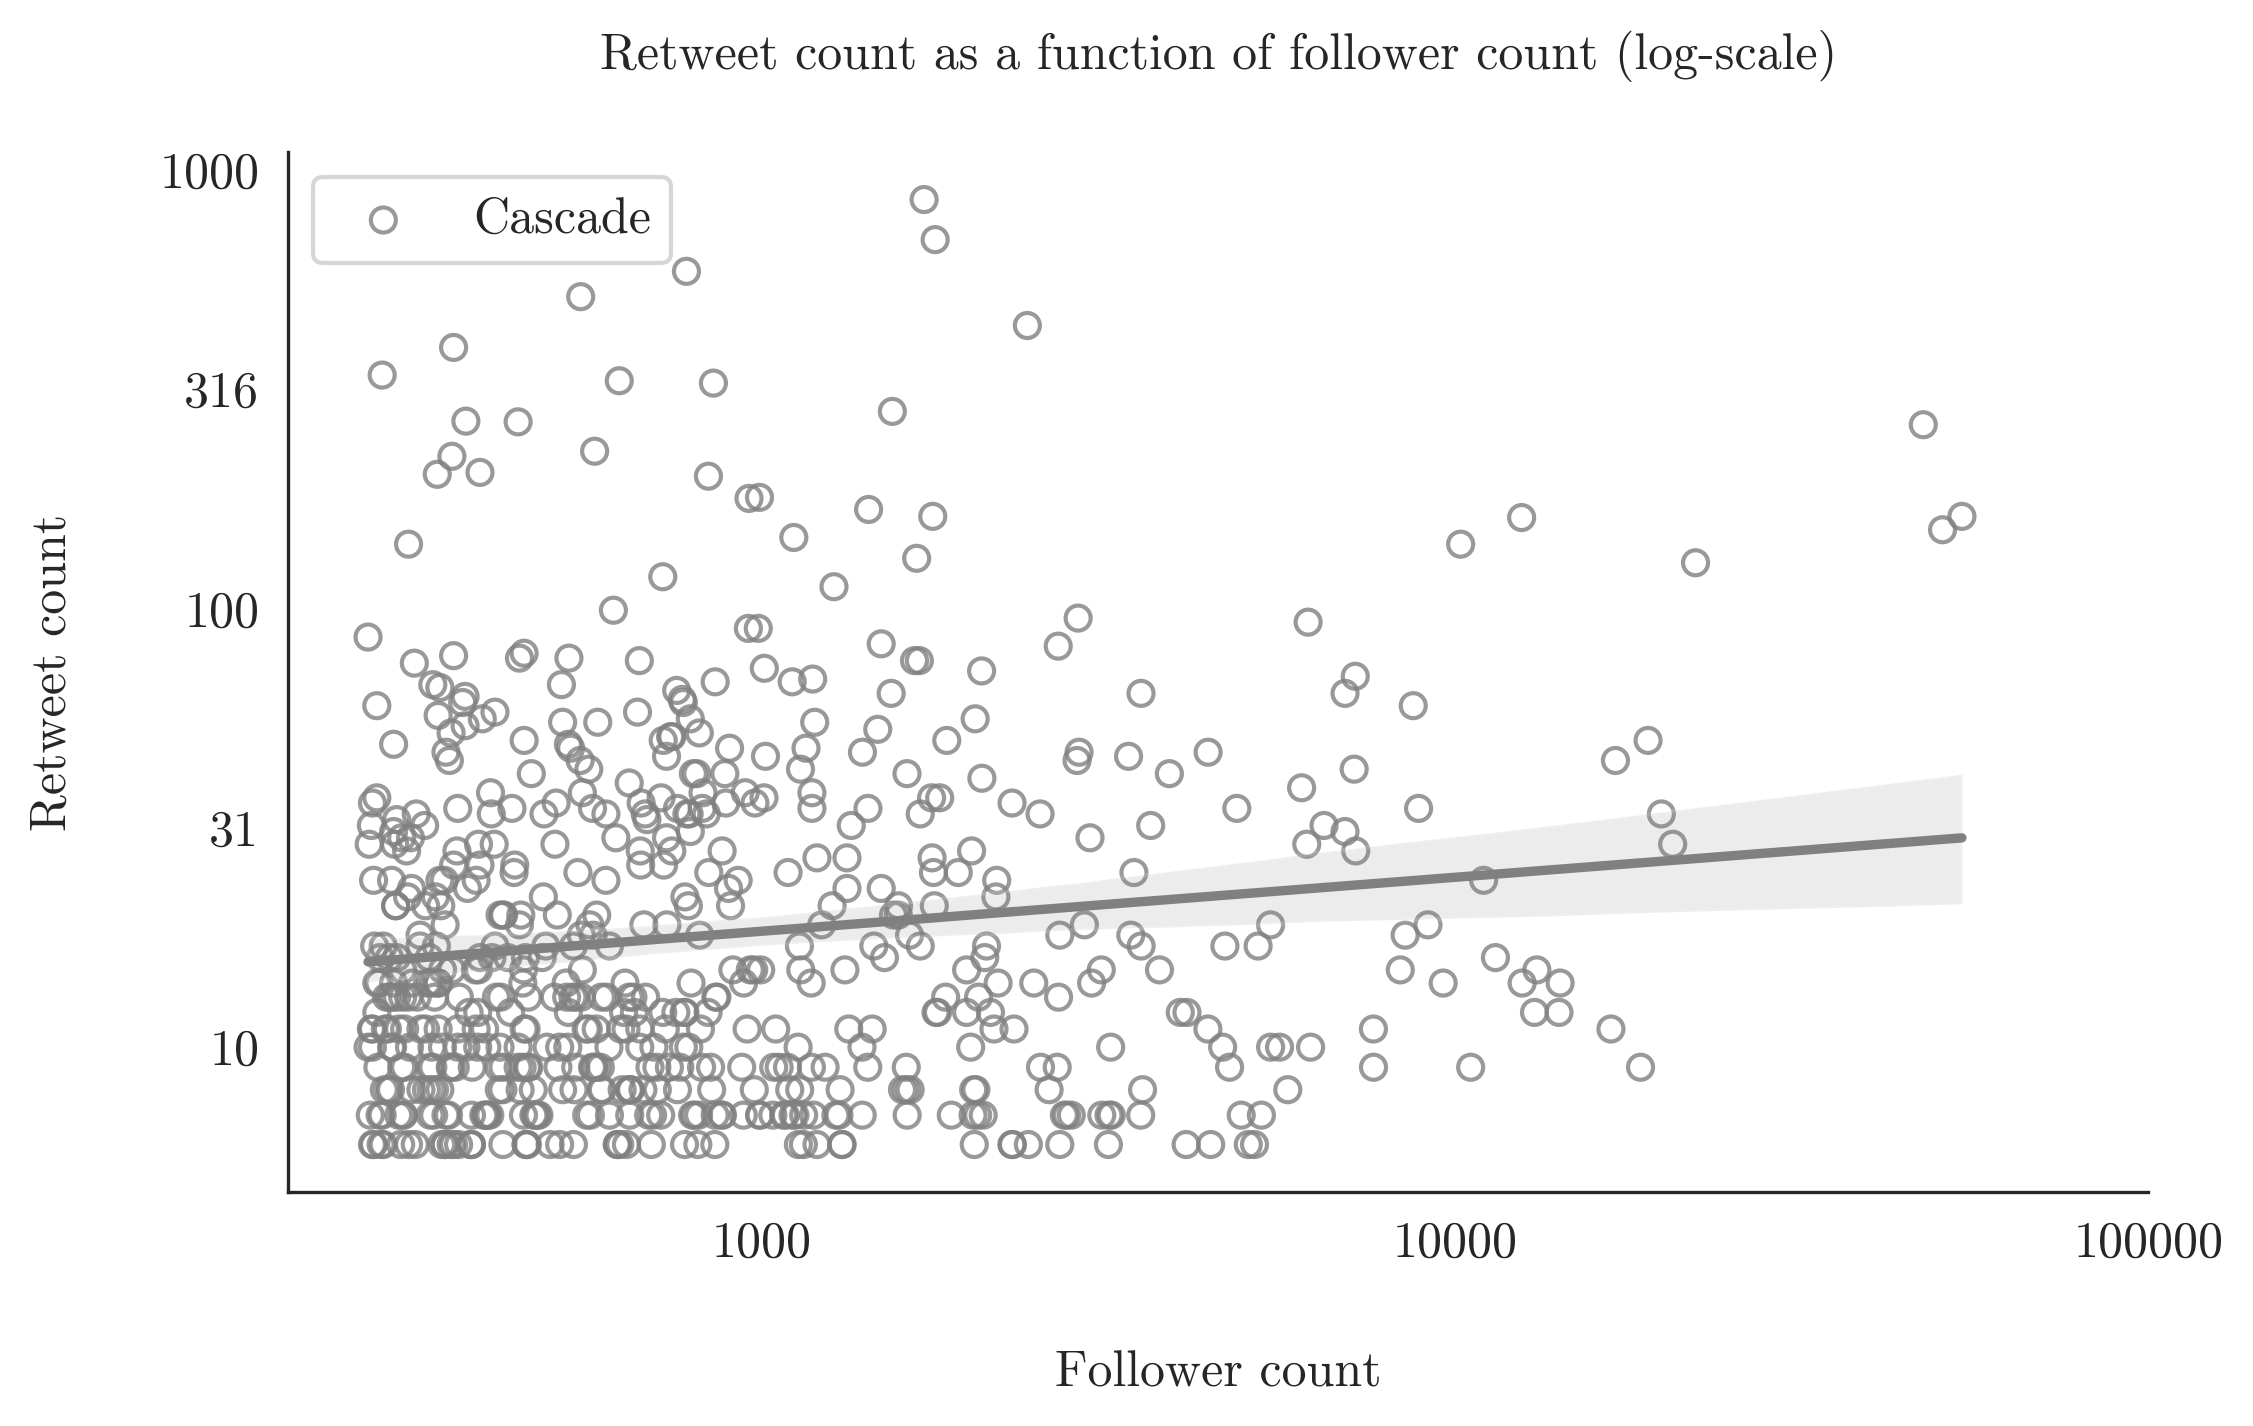
\includegraphics[width=1\linewidth]{linreg_plot.png}\\
        \caption{Null model. Simple linear regression plot (log-scale) showing retweet count as a function of follower count for each cascade. Translucent bands covering the regression line represent 95\% confidence interval. Each circle corresponds to a cascade.}    
        \label{fig:enter-label}
    \end{figure}

    Mean-field SI model was used as the simplest compartmental model of this study. \hyperlink{fig:base-SI}{Figure 5} shows a poor fit between mean-field SI model's predictions and actual retweet count, mainly driven by the very small beta estimate, $\beta = 3.3 \times 10^{-5}$, $R^2 = 0.02$, $MAD = 32.47$. This figure is dominated by simulated retweet counts (y-axis) at the bottom of the graph, as a result of average effect of mean-field models.
    
    \begin{figure}[H]
        \hypertarget{fig:base-SI}{}
        \centering
        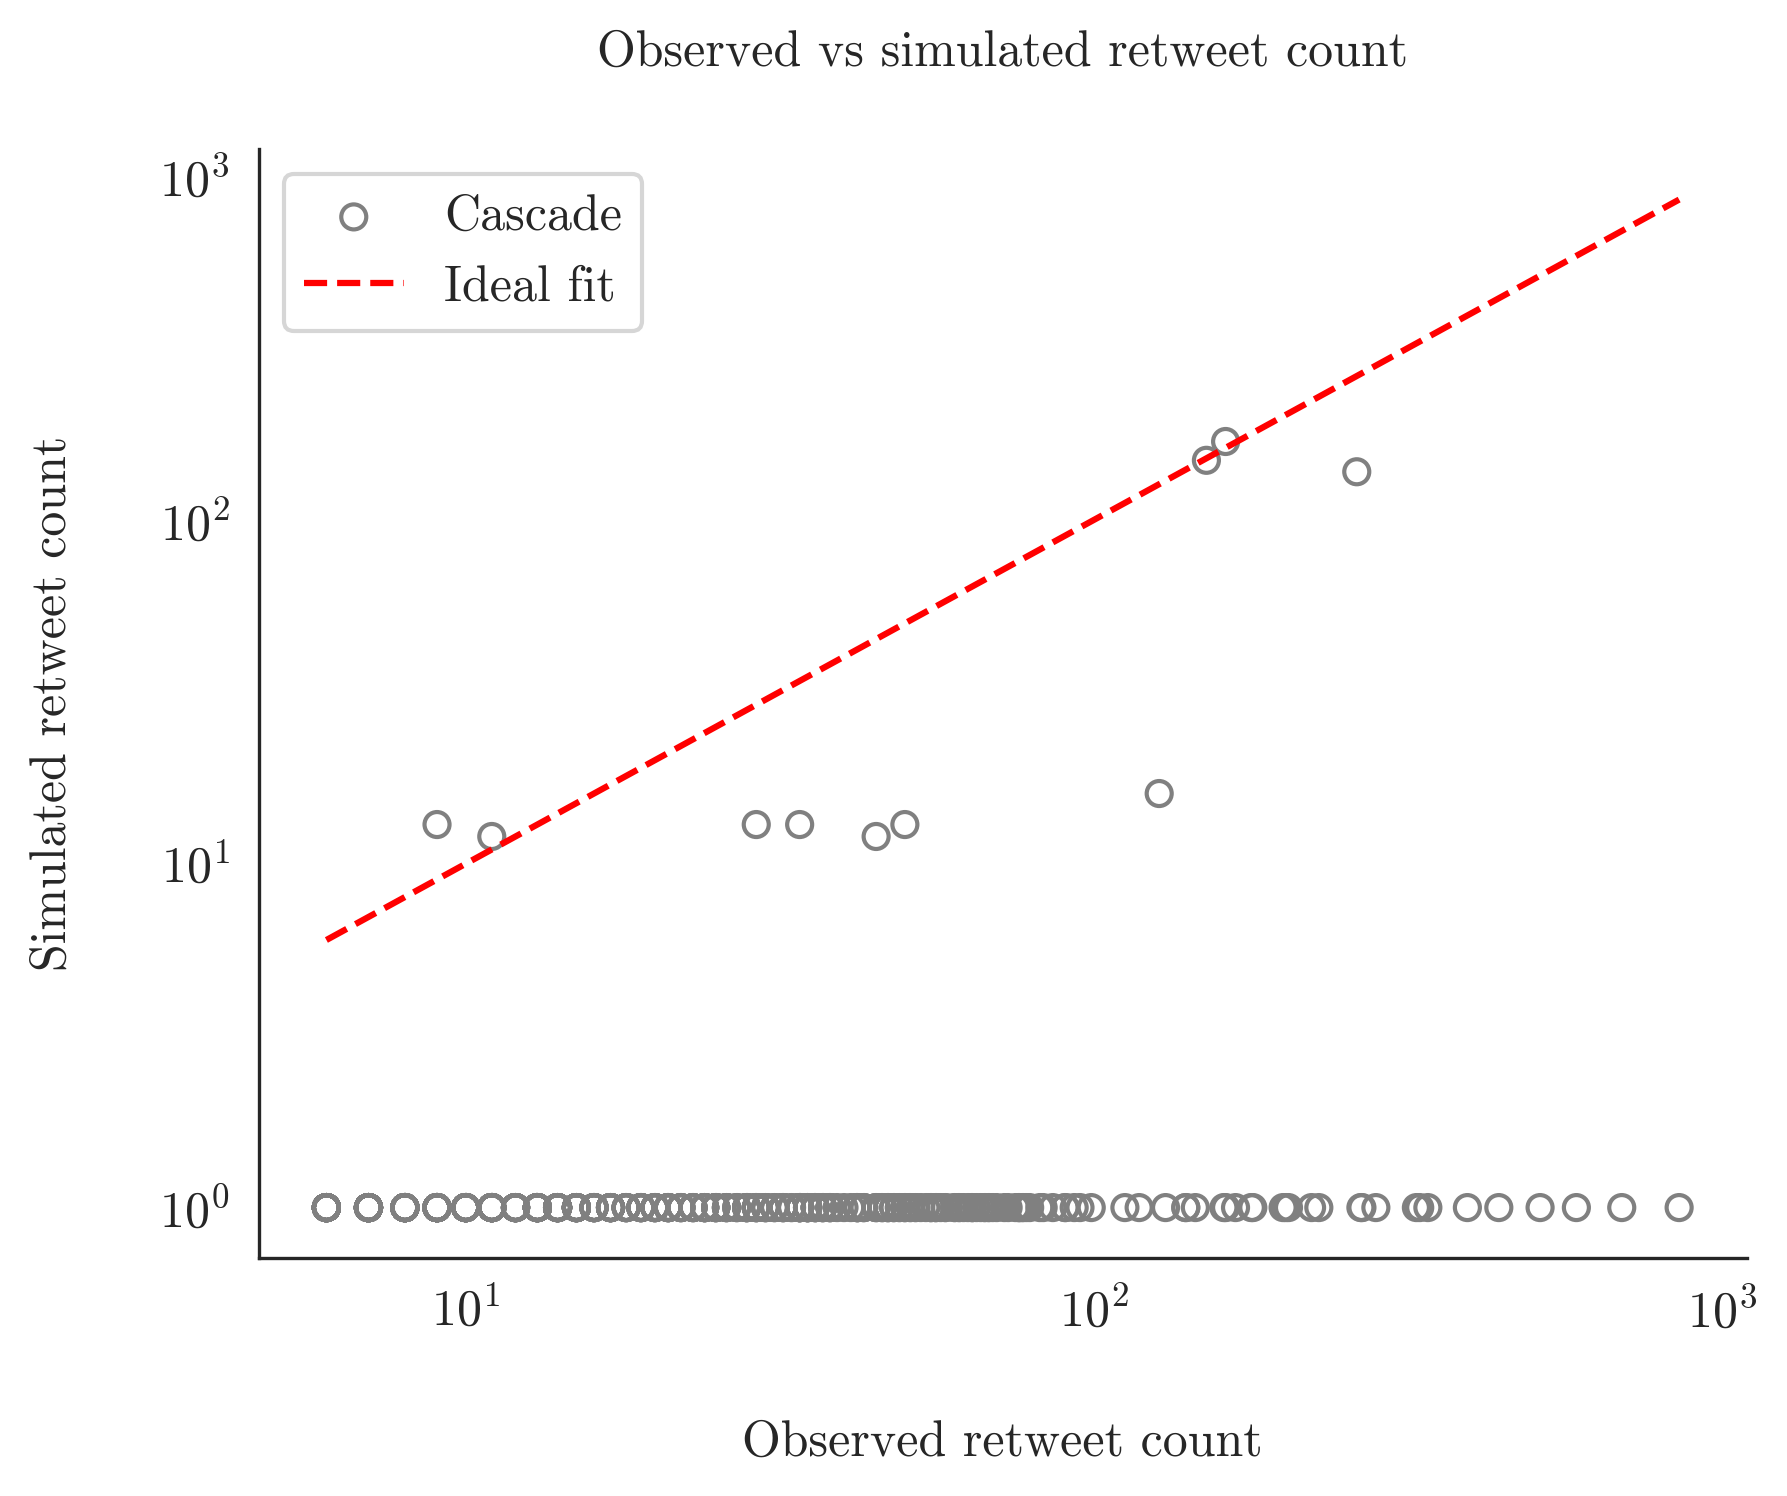
\includegraphics[width=1\linewidth]{thesis/simulate_base_SI_plot.png}\\
        \caption{Mean-field SI model. Scatter plot (log-scale) showing observed and predicted retweets counts for each cascade using mean-field SI model $(\beta = 3.3 \times 10^{-5})$. Red dashed line ($x=y$) corresponds to an ideal fit (i.e., model prediction is the same as observed retweet count).}
        \label{fig:enter-label}
    \end{figure}
    
    Then, network-based SI model was fit. Retweet counts of each cascade were compared with model's predictions, $\beta = 0.001$, $R^2 = 0.018$, $MAD = 29.56$ (\hyperlink{fig:SI}{Figure 6}). Network-based SI model has provided improvement over mean-field model. Yet, the model predictions were still far from an ideal fit (red dashed line).
    
    \begin{figure}[H]
        \hypertarget{fig:SI}{}
        \centering
        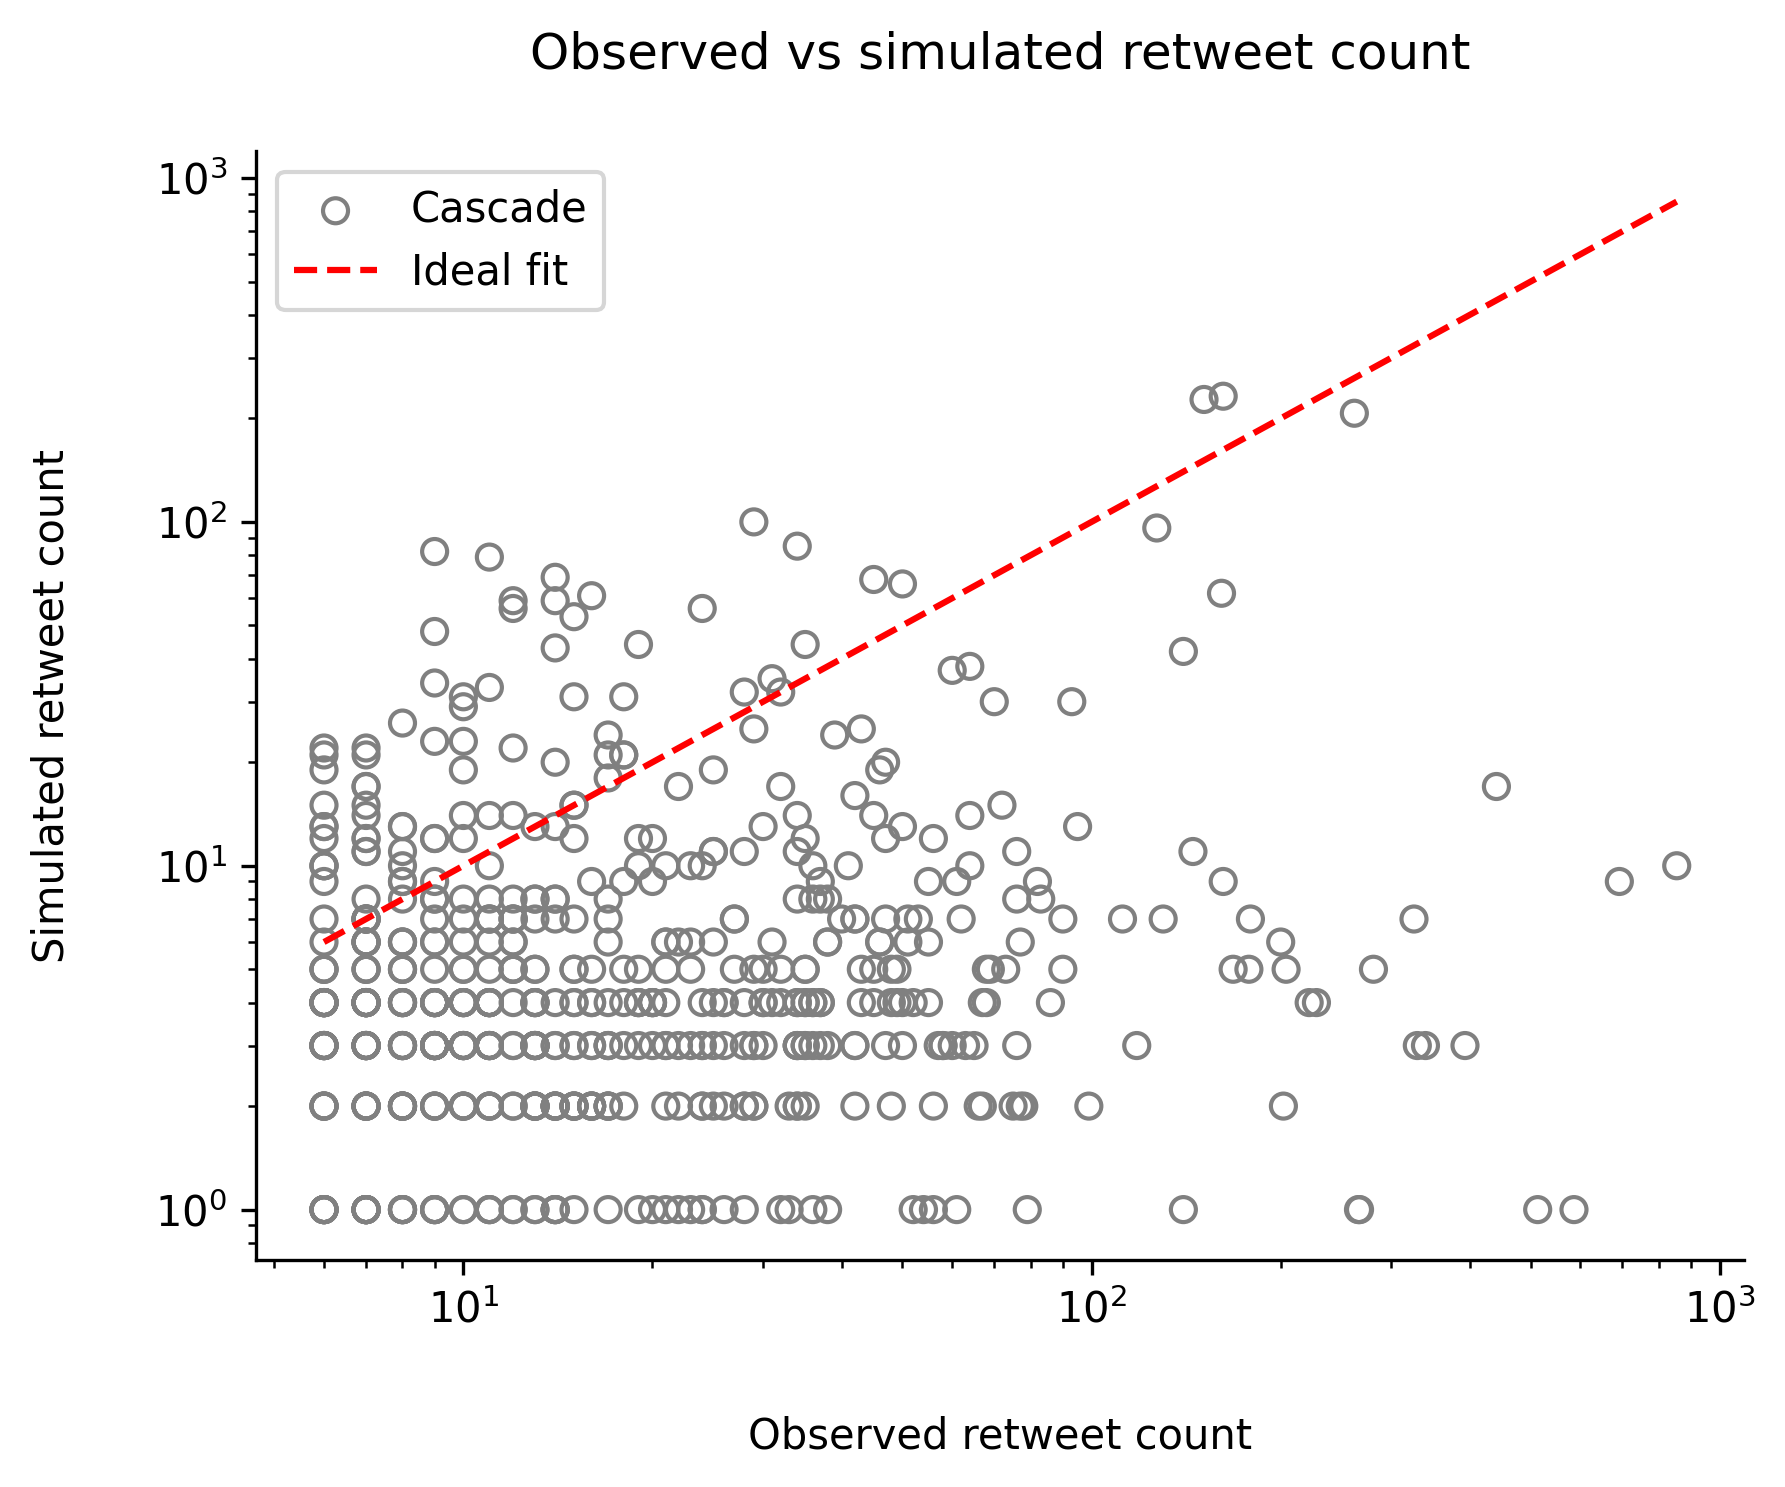
\includegraphics[width=1\linewidth]{thesis/simulate_SI_plot.png}\\
        \caption{Network-based SI model. Scatter plot (log-scale) showing observed and predicted retweets counts for each cascade using SI model $(\beta = 0.001)$. The red dashed line ($x=y$) corresponds to an ideal fit where, model prediction is the same as observed retweet count.}    
        \label{fig:enter-label}
    \end{figure}
    
    Given the subpar results of SI models, IC model, which has more realistic assumptions about the data were fit. IC model showed no significant improvement in model fit, $p_{uv} = 0.003$, $R^2 = 0.016$, $MAD = 29.74$, in comparison to the SI model. Surprisingly, \hyperlink{fig:IC}{Figure 7} (IC model) shows a very similar plot to \hyperlink{fig:SI}{Figure 6} (SI model).
    
    \begin{figure}[H]
        \hypertarget{fig:IC}{}
        \centering
        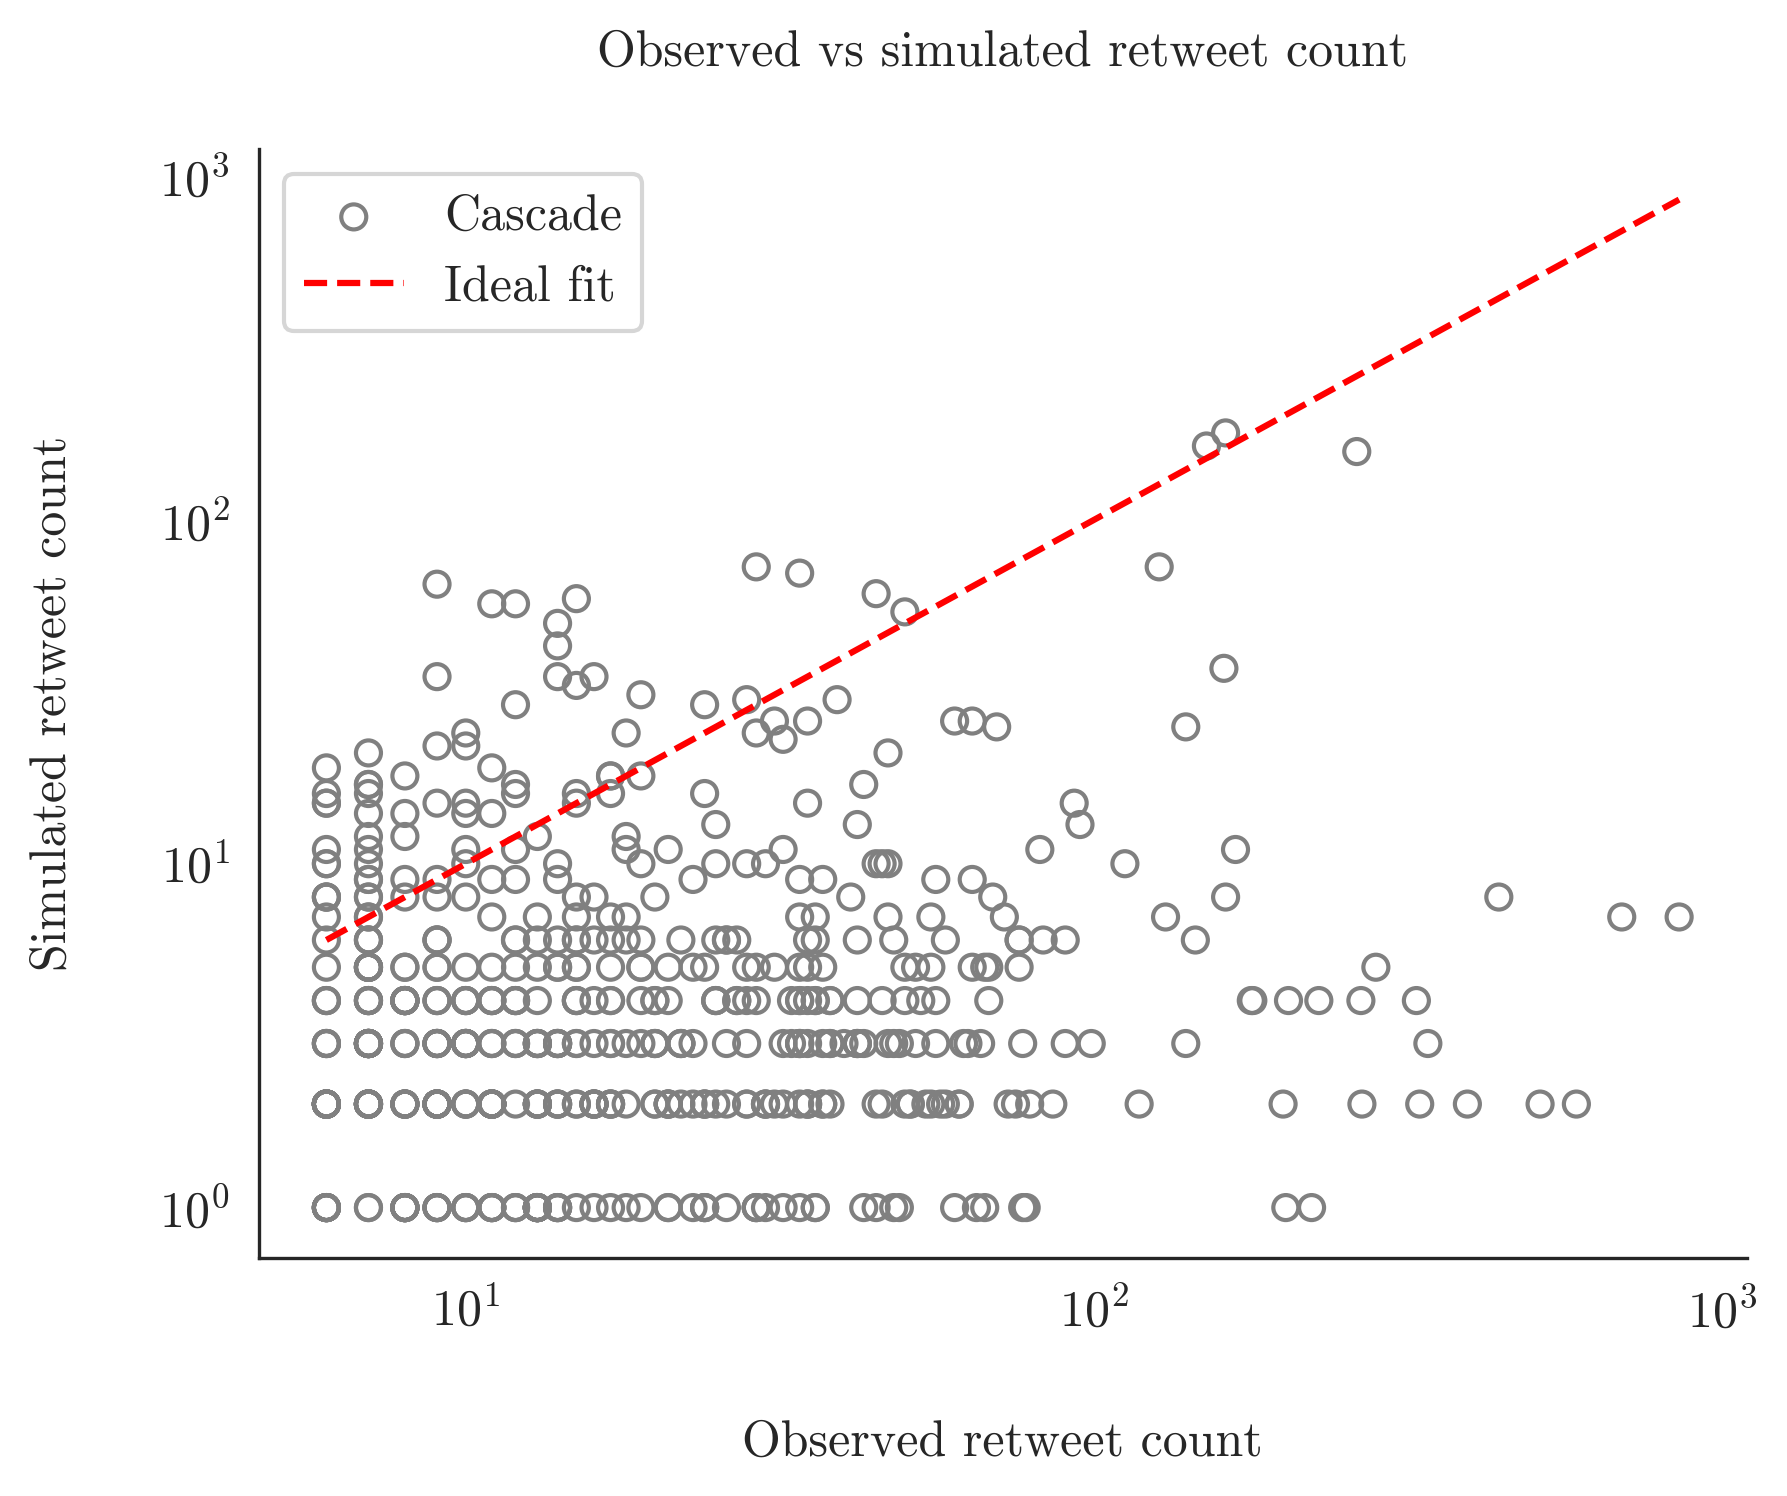
\includegraphics[width=1\linewidth]{thesis/simulate_IC_plot.png}\\
        \caption{Independent Cascades model. Scatter plot (log-scale) showing observed and predicted retweets counts for each cascade using IC model ($p_{uv} = 0.003$). The red dashed line $(x=y)$ corresponds to an ideal fit, where model prediction is the same as observed retweet count.}    
        \label{fig:enter-label}
    \end{figure}

    IC model was extended to incorporate an infectiousness parameter that goes under an exponential decay. Results show no significant improvement over the IC model, $p_{uv} = 0.003$, $\lambda = 0.94$, $R^2 = 0.019$, $MAD = 29.69$ (\hyperlink{fig:dec-IC}{Figure 8}). Even though there was no significant improvement in model fit, decaying IC model was also used to generate the cumulative distribution of retweet count over model iterations in \hyperlink{fig:ecdf-vs-iter}{Figure 9}.
    
    \begin{figure}[H]
        \hypertarget{fig:dec-IC}{}
        \centering
        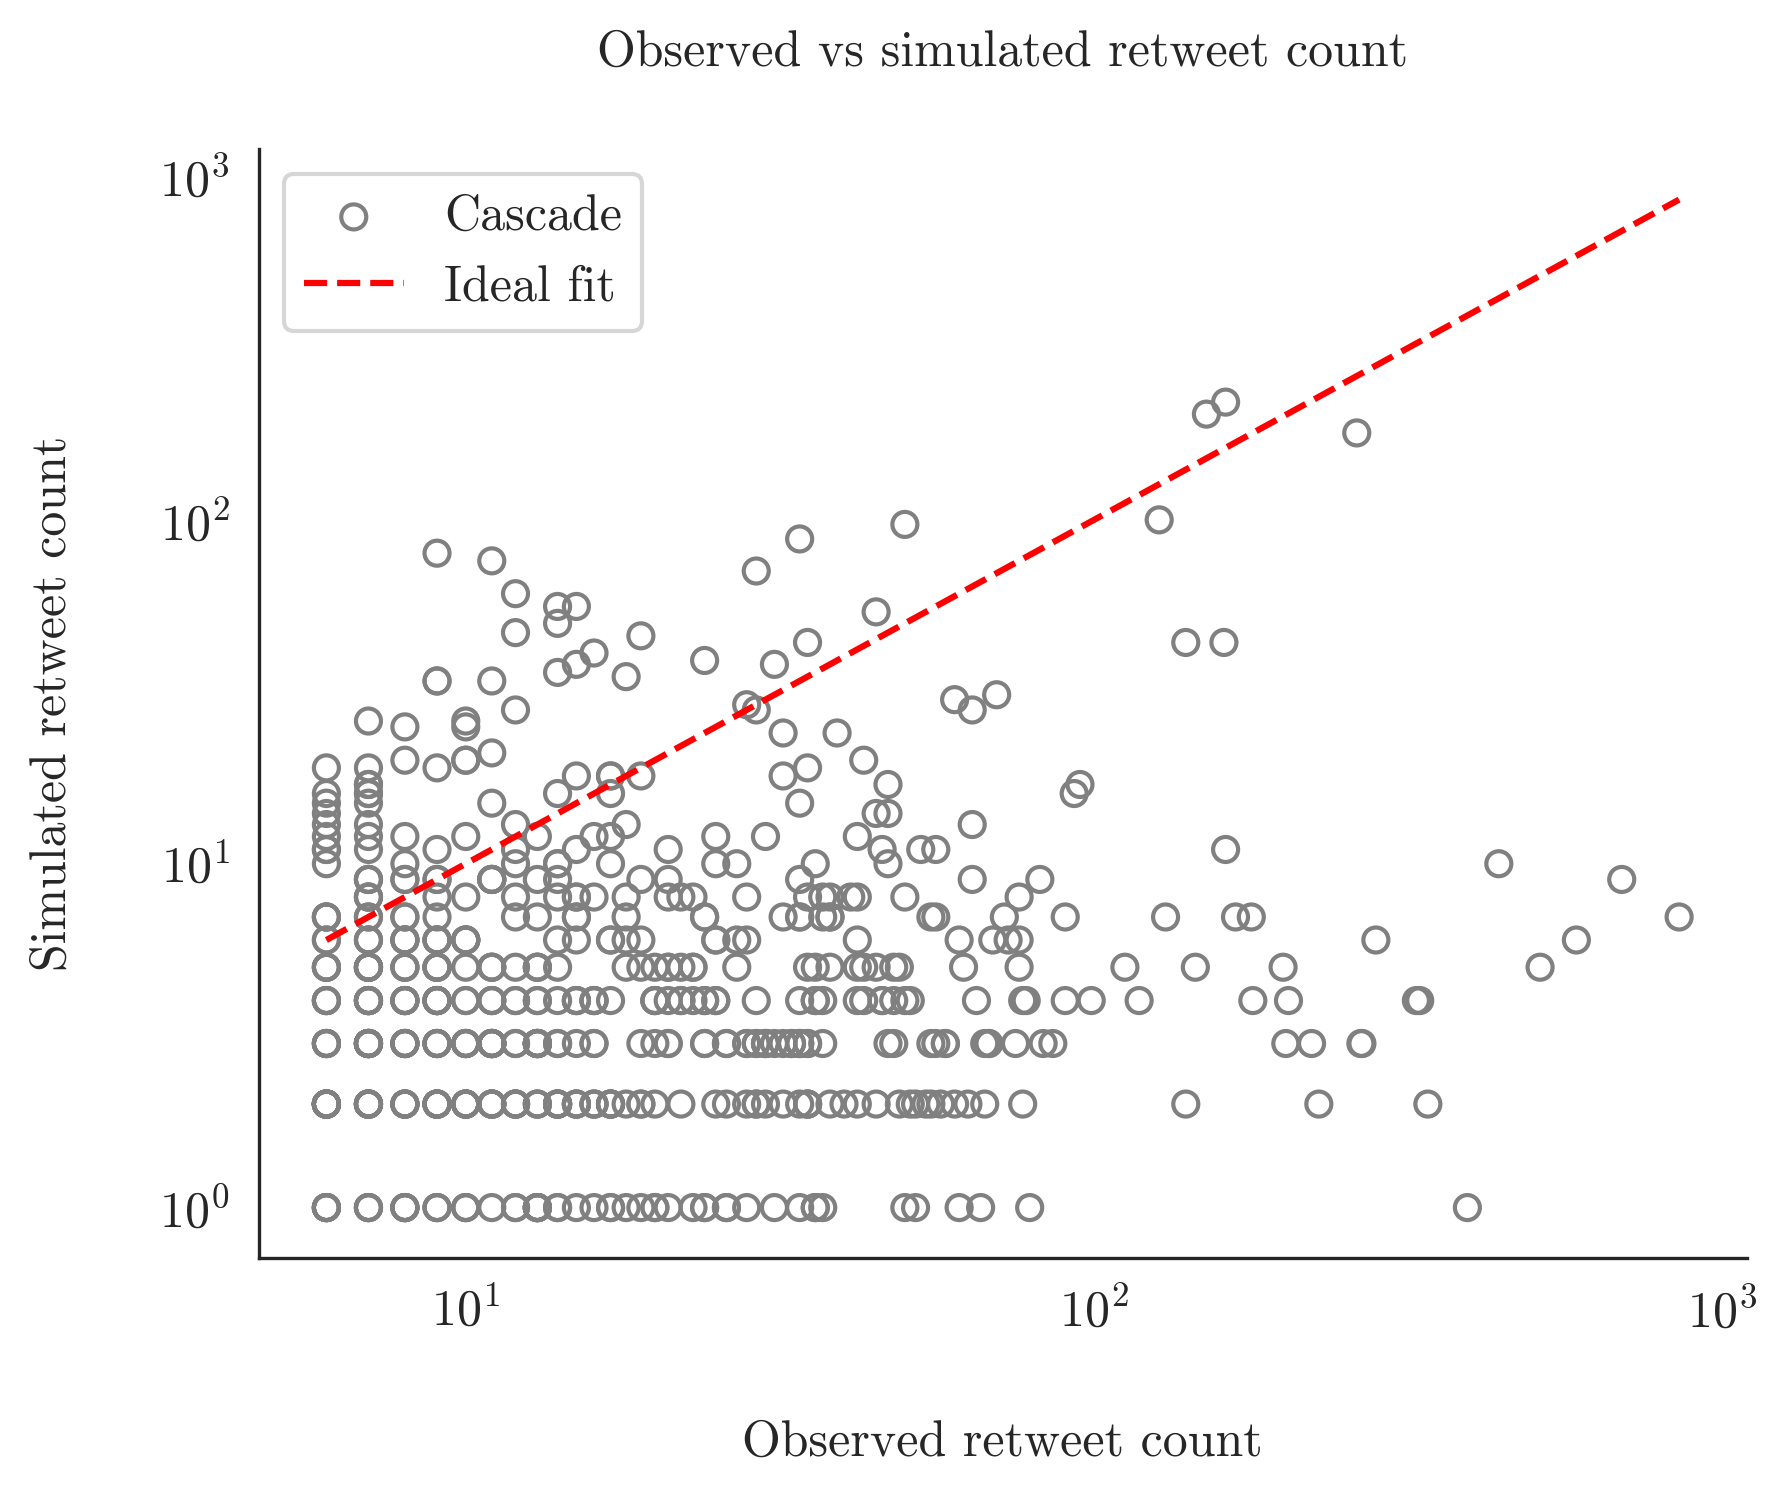
\includegraphics[width=1\linewidth]{thesis/sim_decaying_IC_plot.png}\\
        \caption{Decaying Independent Cascades model. Scatter plot (log-scale) showing observed and predicted retweet counts for each cascade using decaying IC model $(p_{uv} = 0.003, \lambda = 0.94)$. The red dashed line ($x=y$) corresponds to an ideal fit where model prediction is the same as observed retweet count.}    
        \label{fig:enter-label}
    \end{figure}

    \hyperlink{tab:comp}{Table 2} summarizes model fit results, and model parameters used to investigate RQ1, that is, modeling final retweet counts of cascades. As can be seen on \hyperlink{tab:comp}{Table 2}, R-squared and MAD values were very close to each other, the only big difference being the null model (i.e., simple linear regression), which had a superior R-squared result.

    \begin{table}[H]
        \hypertarget{tab:comp}{}
      \centering
      \begin{tabular}{|l|l|l|l|}
        \hline
        \textbf{Model} & \textbf{R-squared} & \textbf{MAD}  & \textbf{Parameters} \\
        \hline
        Null model    & 0.13 & 31.16 & $a = 0.002$, $b = 30.41$  \\
        Mean-field SI & 0.02 & 32.74 & $\beta = 3.3 \times 10^{-5}$ \\
        Network-based SI & 0.018 & 29.56 & $\beta=0.001$ \\
        IC               & 0.016 & 29.74 & $p_{uv} = 0.003$  \\
        Decaying IC      & 0.019 & 29.69 & $p_{uv} = 0.003$, $\lambda = 0.94 $ \\
        \hline
      \end{tabular}
      \caption{Model comparison table for RQ1}
      \label{tab:mytable}
    \end{table}

    \subsection{RQ2}
    ECDFs were computed for capturing temporal properties of retweet cascades. \hyperlink{fig:ecdf-vs-iter}{Figure 9} [left] features fifteen ECDF plots showing the temporal evolution of fifteen cascades. As can be seen on \hyperlink{fig:ecdf-vs-iter}{Figure 9}, cascades show that the life-cycle of a tweet is short and characterized by rapid burst in the first few hours, followed by a slow and steady expansion thereafter.
    
    After visually inspecting ECDF plots, plans for fitting a \hyperlink{sec:sigmoid}{sigmoid function} was abandoned and logarithm function was identified to be a better fit (\hyperlink{eq:avrami}{Equation 10}). 
    
    \hyperlink{fig:ecdf-vs-iter}{Figure 9} [right] also features model simulations for the same set of fifteen cascades. For most tweets, more than 50\% of all retweets a cascade will experience are simulated in the first model iteration. Almost all cascades reach their 100\% retweet ratio within the second iteration of the model. Third iteration is the final iteration of the model and all cascades complete their life-cycle by then.

    Both graphs were featuring a logarithmic shape. Hence a logarithm function was fit to the empirical cumulative distribution on the left,  $a = 0.17$, $b =  0.77$. As well as to the cumulative distribution of retweet counts over model iterations on the right, $a = 0.24$, $b =  0.70$.

    \begin{figure}[H]
        \hypertarget{fig:ecdf-vs-iter}{}
        \centering
        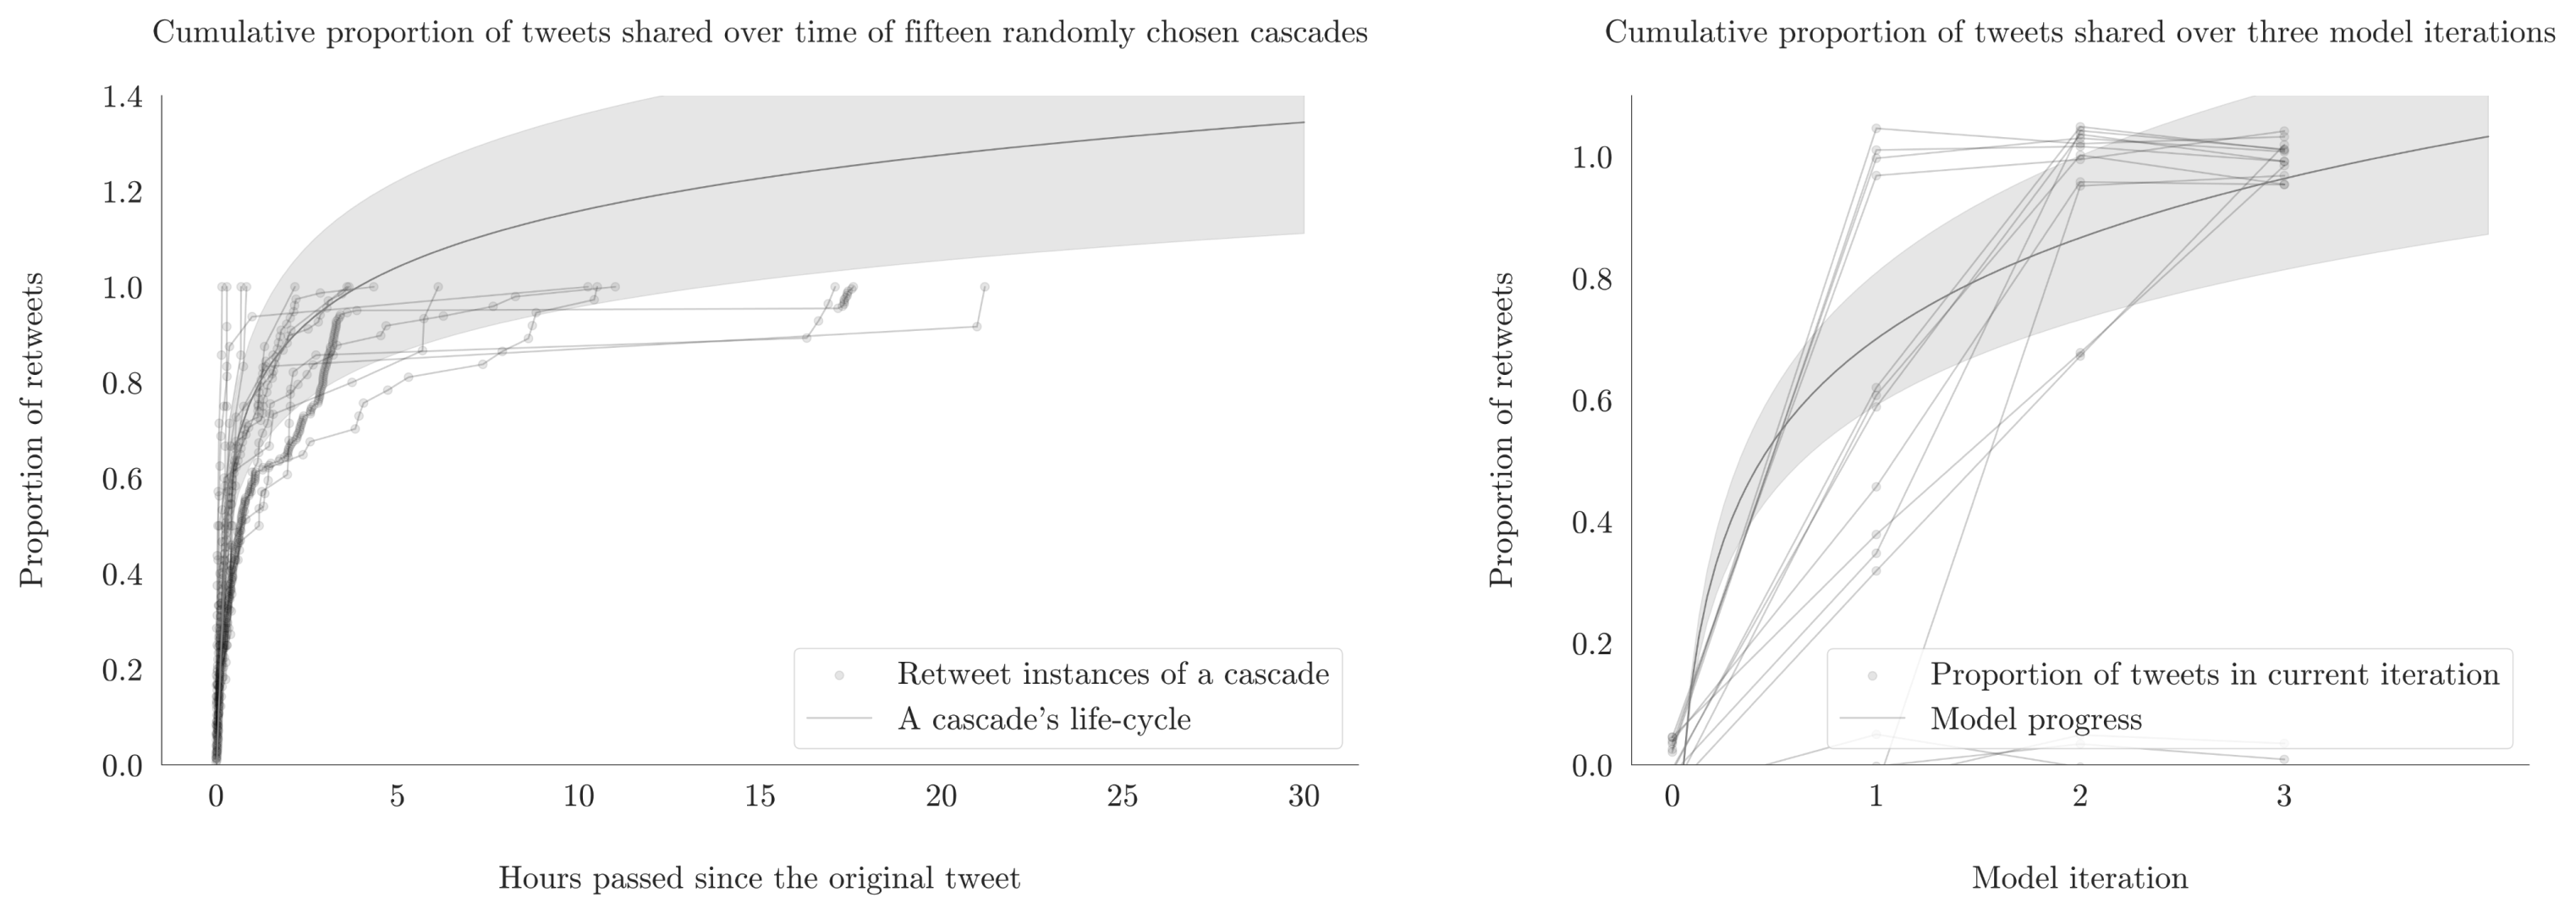
\includegraphics[width=1\linewidth]{thesis/ecdf_vs_model_iter.png}\\
        \caption{[Left] Connected dots: Empirical cumulative distribution function plots for fifteen randomly chosen cascades showing the percentage of total retweets sent by the given time point. Large gaps between dots signify the time gap between the first burst of retweets and the subsequent retweets. Gray line: Logarithmic fit estimated by fitting a logarithmic equation to all the cascades. Error bands were calculated by multiplying mean absolute deviation with y-values and  adding, subtracting from y-values. [Right] Decaying IC Model simulations for the same set of fifteen cascades. Connected dots signify the ratio of retweets sent in a cascade by the given model iteration. Error bands for the cumulative distribution of the decaying IC model are calculated the same way.} 
        \label{fig:enter-label}
    \end{figure}

    \hyperlink{tab:comp2}{Table 3} summarizes model fit results, and model parameters used to investigate RQ2, that is, modeling final retweet counts of cascades. As can be seen on \hyperlink{tab:comp}{Table 3}, $a$ and $b$ (\hyperlink{eq:log}{Equation 11}) values were very close to each other.

    \begin{table}[H]
        \hypertarget{tab:comp2}{}
      \centering
      \begin{tabular}{|l|l|l|l|}
        \hline
        \textbf{Logarithm function fitted on} & \textbf{a} & \textbf{b} \\
        \hline
        ECDF    & $0.17$ & $0.77$   \\
        Decaying IC & $0.24$ & $0.70$ \\
        \hline
      \end{tabular}
      \caption{Comparing logarithm function model parameters (\hyperlink{eq:log}{Equation 11}) RQ2}
      \label{tab:mytable}
    \end{table}

    \subsection{RQ3}
        The dataset had a skewed distribution of topics, leaving some topics underrepresented in the data (\hyperlink{fig:topic-dist}{Table 4}).
        
        \begin{table}[h]
        \hypertarget{fig:topic-dist}{}
        \centering
        \begin{tabular}{|l|l|l|}
            \hline
            \textbf{Topic} & \textbf{Count} & \textbf{Infectiousness ($p_{uv}$)} \\
            \hline
            Relief efforts, resources, donations, and infrastructure & 229 & 0.004 \\
            Impact, aftermath, death toll & 98 & 0.006 \\
            International response and international support & 79 & 0.011 \\
            Controversy, criticism, social and political commentary & 58 & 0.005 \\
            Rescue operations and assistance & 30 & 0.005 \\
            Faith and prayers & 30 & 0.005 \\
            Personal experience, stories, and missing people & 27 & 0.006 \\
            Aftershocks and tremors & 23 & 0.001 \\
            Technology, communication, and social media & 19 & 0.012 \\
            The tweet does not fit any of the given topics. & 12 & 0.008 \\
            \hline
        \end{tabular}
        \caption{List of topics, cascade counts, and their infeciousness, measured by the $p_{uv}$ parameter of the IC model.}
        \end{table}
    
        A one-way ANOVA was conducted to compare the retweet counts among ten topic clusters. Despite the lack of a statistical significant result, $F (9, 595) = 1.61$, $p = 0.11$, two topics exhibited noticeable distinctions in their infection rates (\hyperlink{fig:topic-comp}{Figure 10}). 
    
        \begin{figure}[H]
            \hypertarget{fig:topic-comp}{}
            \centering
            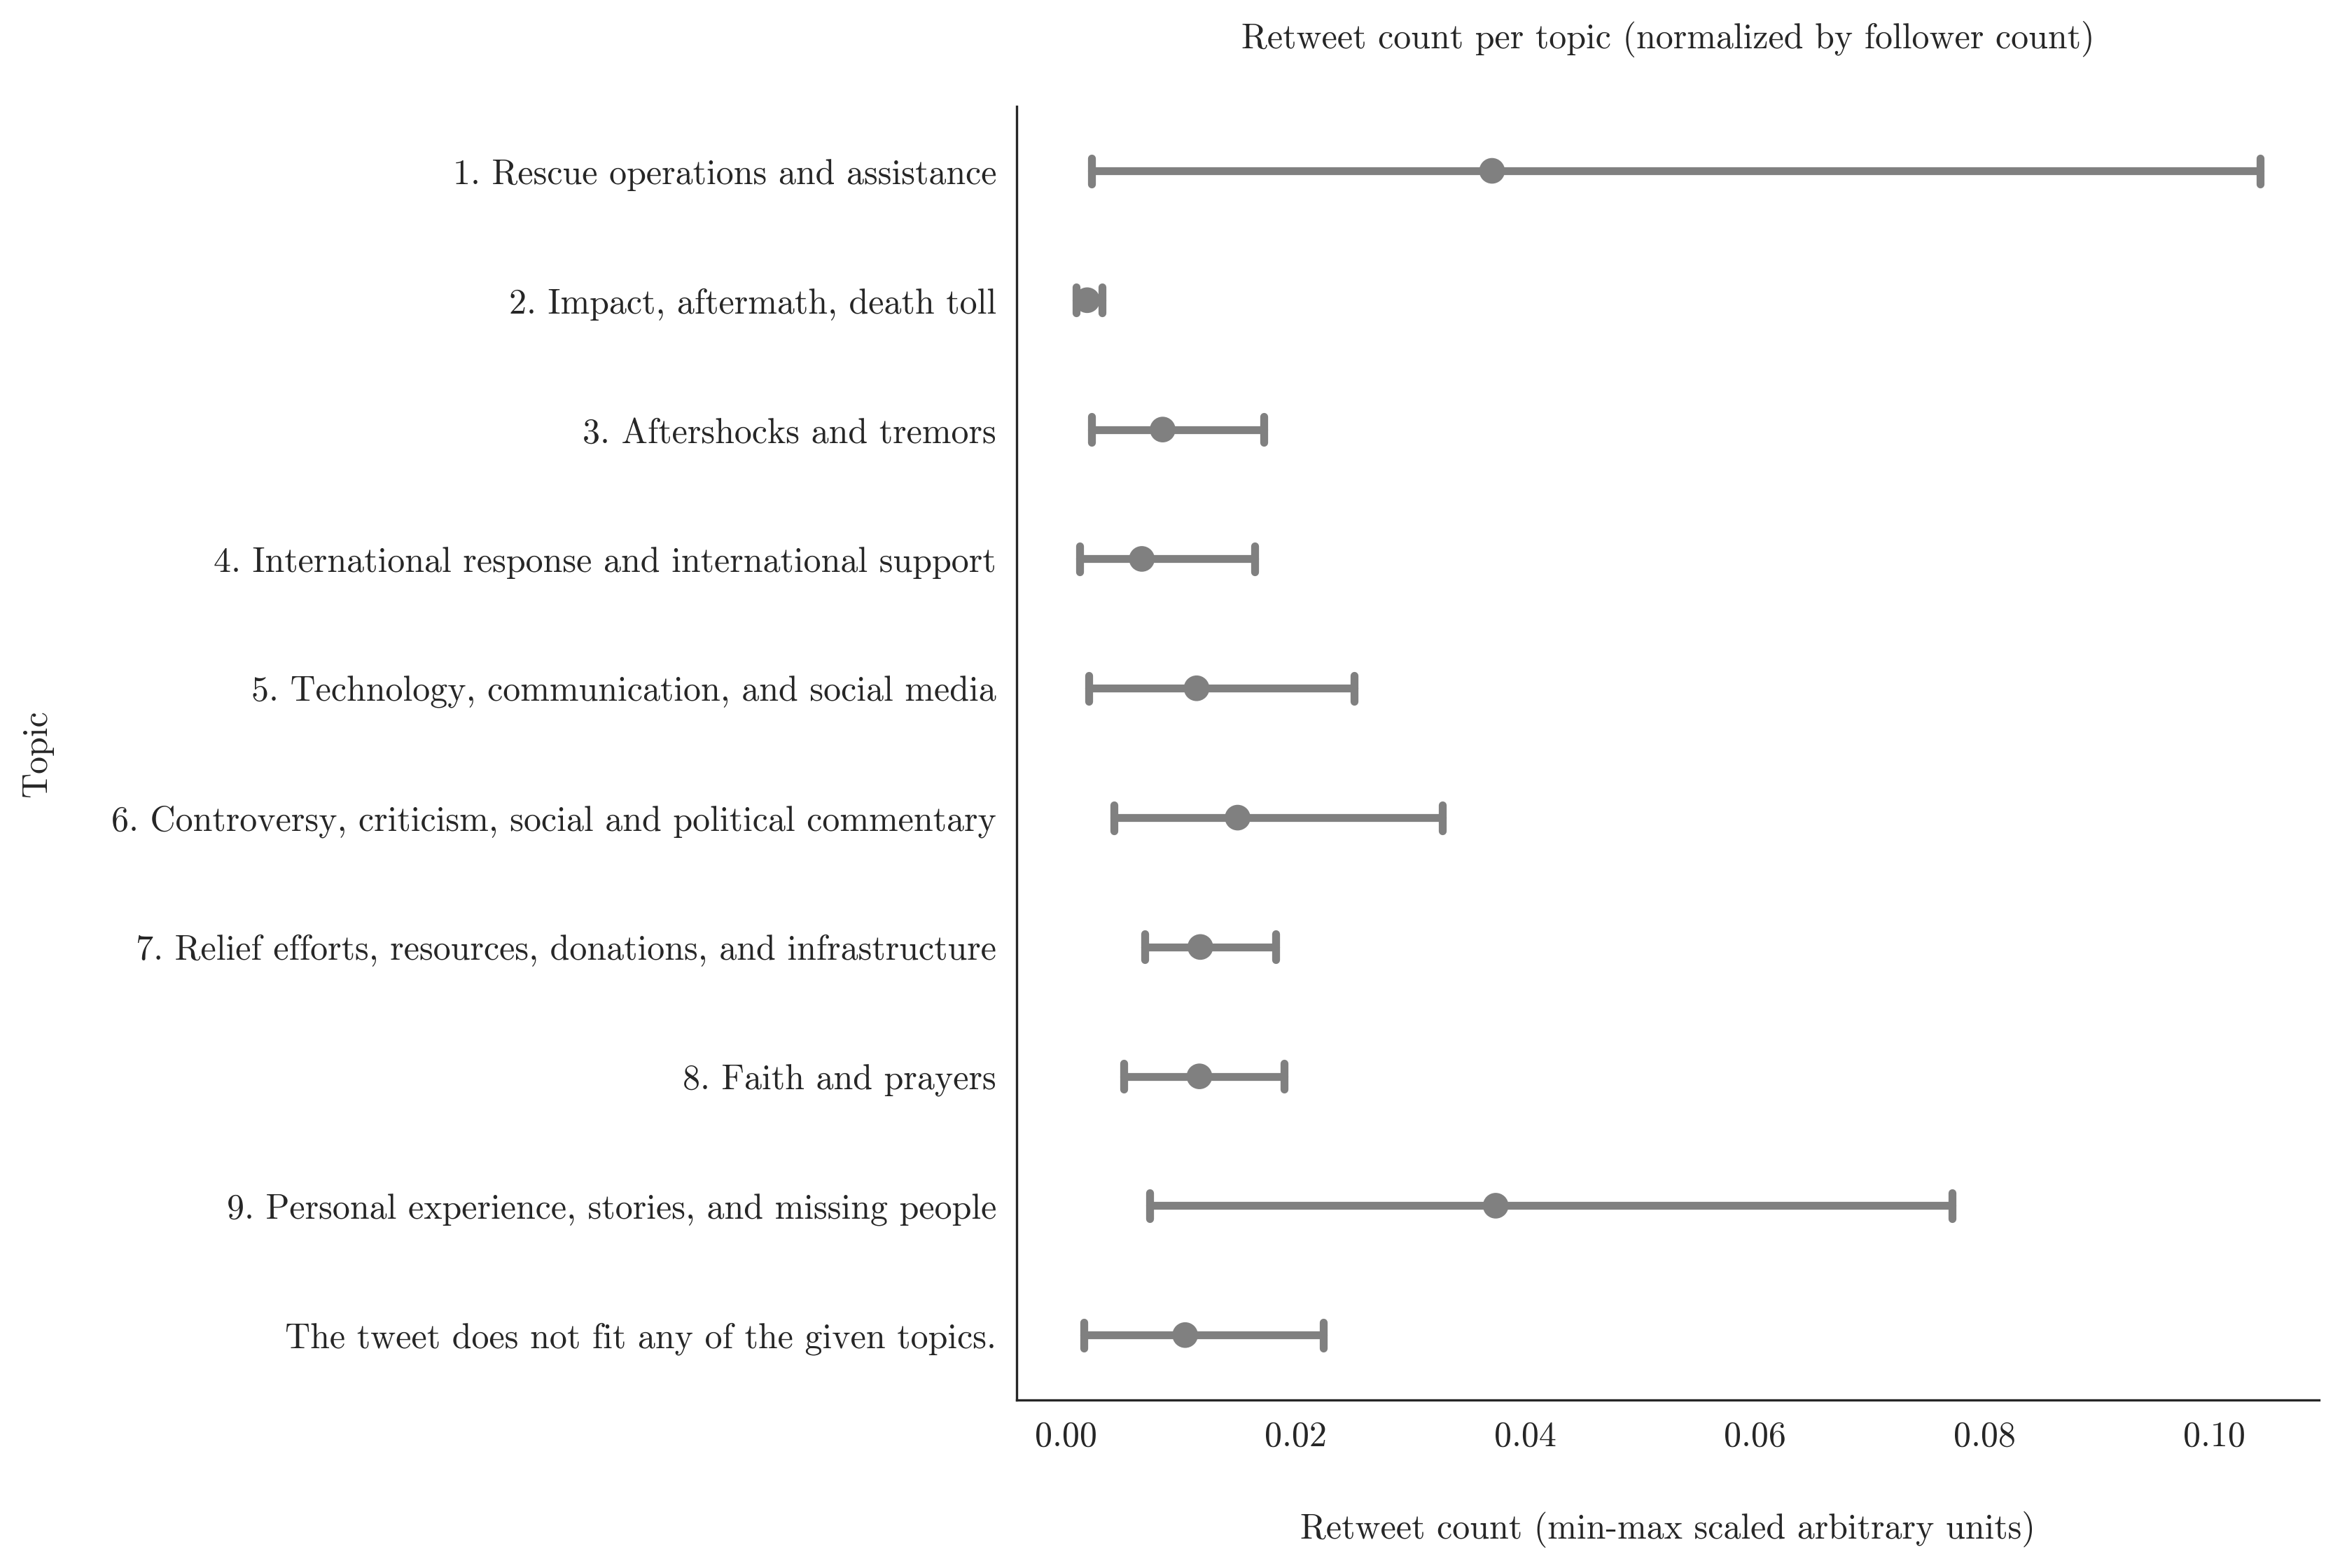
\includegraphics[width=1\linewidth]{topic_n_rt_norm_plot.png}\\
            \caption{Point plot showing the mean retweet count for each topic in arbitrary units. Error bars represent standard deviation.}        
            \label{fig:enter-label}
        \end{figure}
    
        Infectiousness parameters between topics were compared. To do that, dataset was broken down into topic categories, then, parameter estimation was done once for each topic. Results show highly variable infectiousness across different topics (\hyperlink{fig:topic-dist}{Table 4}) and that the most infectious topics are \textit{International response and international support} and \textit{International response and international support} Infectiousness is only presented as a point estimate, and standard deviation is not reported. Because bootstrapping samples to measure variability was attempted but the computation time was becoming unfeasible.
        
        Data were also classified according to its semantic categories (factual vs emotional). More tweets were classified as factual $(n = 396)$ than emotional/personal $(n = 199)$. Comparing retweet count across two categories did not yield significant results, $T(603) = 1.64$, $p = 0.10$.

        Nonetheless, just as with the topic, semantic categories were also compared in terms of their infectiousness. Results showed that emotional/personal tweets had lower infectiousness ($p_{{uv}_{emo}} = 0.004$) than factual tweets ($p_{{uv}_{fact}} = 0.005$).
        
%%%%%%%% DISCUSSION %%%%%%%%
\clearpage
\section{Discussion}
    
    In this study, I investigated the information diffusion on Twitter by modeling the retweet count and time series behavior of tweet cascades. Attempts were also made to break down the dataset into categories. The following sections repeat and discuss the results of the study at hand.
    
    \subsection{RQ1}
    Five models with increasing complexity and more realistic assumptions were fit to the data to model retweet count. First, best fitting model parameters were estimated. Then, simulations were run. Finally, simulated and observed retweet counts were compared to evaluate model fit.
    
    The null model predicted the retweet count with a simple linear regression based solely on follower count and had a very modest performance. The null model served as a benchmark to test usefulness of more complex models. Compared to other models, the null model was much easier to deploy, required much less computational resources and only a very basic data about the cascades, that is, the number of followers. Hence, models featured in the rest of this section were expected to outperform the null model to justify for their complexity, computational costs, data needs.
    
    Mean-field SI model has performed worst, likely because of the average mean-field effect. Since the model assumes that all agents have a chance to interact with each other over all the iterations the estimated $\beta$ values were chosen to be a minuscule. If a larger $\beta$ value was to be chosen, the model was heavily overestimating the number of retweets. This effect gets more profound when I factored in the number of iterations. Over four iterations, where each and every node interact with each other, the number of interactions rise exponentially. Thus, $\beta$ value was chosen to be very small, causing many cascades to have zero simulated retweets (\hyperlink{fig:base-SI}{Figure 5}).
    
    The network-based SI model yielded improvements above its mean-field counterpart and the null model, strengthening the case for incorporating network structure to understand diffusion dynamics. In the network-based version, network structure was taken into account so that the number of possible interactions were greatly reduced. As a consequence, $\beta$ value in this model could increase to meaningful range. Network-based SI model was not free of limitations. Infected nodes were able to infect susceptible nodes on every iteration. This, however, does not reflect information diffusion dynamics on Twitter, where interactions between nodes are mostly one-time events instead of recurring over iterations.
    
    The IC model addressed the shortcoming of the SI model by changing the rule of how nodes interact with each other. The IC model limits the interaction instances between each node pair to one. In other words, each infected node has only one chance to infect each of its neighbors. If it fails to infect its neighbor, no further interactions take place within this node dyad. This dynamic much closely resembles the dynamics on Twitter. As discussed previously, selecting number of iterations is under the modeler's discretion. IC model allows the modeler to choose a high iteration count for the model without having to sacrifice accuracy with deflated infectiousness values. This means model can run for longer and potentially capture nodes with higher path length. For instance, if the number of iterations is set to 3, the model runs for three iterations and the maximum path length a node can have is 3. If the number of iterations is set to, say, 6, source node can, in turn, affect a node that requires 6 jumps from the source node. Hence the information diffusion can go deeper. In network-based SI model, increasing the model iteration would cause the beta value to go down. Consequently network-SI model would run into the same problem with mean-field SI model, where a minuscule beta value caused most simulations to be zero.
    
    To my surprise, the IC model provided little to no improvement over the SI model. This can be explained by the fact that almost all the retweets a cascade receives comes from the first iteration, that is, from followers of the source node (\hyperlink{fig:ecdf-vs-iter}{see Figure 9}). Put differently, most cascades in the dataset received most of their retweets during the second interation. Suppose cascade $c$ has been retweeted a hundred times, $rt_{total} = 100$. A very large portion of these retweets in fact come from the first iteration ($rt_1 = 90$), where only the original poster is making her followers retweet. The rest of the retweets ($rt_{total-1} = 10$) comes from the other three iterations. In short, the first iteration explains most of the variance in model simulations and the subsequent iterations have only limited effect on model simulations. Thus, the IC model, although is theoretically superior to the SI model, provided little to no improvement over SI model.
    
    Previous literature has refuted the hypothesis that the infectiousness parameter ($\beta$ or $p_{uv}$) stays constant across model iterations \cite{goel_note_2015}. In other words, unlike some viral infections, the infectiousness parameter starkly declines after the first iteration. Henceforth, in this study, I added an exponential decay parameter to the IC model to overcome this drawback. Nevertheless, the decaying IC model offered a negligible improvement over the IC model. In short, model complexity had little benefit on model fit scores. Again, this can be explained by the reason stated in the above paragraph.
    
    Modeling retweet count with increasing model complexity and more realistic assumptions showed inconsistent improvements in model fit going from null model to decaying IC model. The reason behind that can be the following: In the case of an epidemic, transmission goes deeper. Meaning that the disease spreads have a much longer path length. A disease can easily go much further beyond the source node. And nodes interact with each other over a longer period of time. Yet, most tweet cascades are, in fact, small and have low depth \cite{goel_structural_2016}. Whereas network-based epidemiology models become more powerful when the underlying network structure is utilized more prominently. For example, a susceptible node that is multiple degrees away from the source node have a substantial chance of getting infected in an epidemic case, but a minuscule probability to retweet.

    Modeling retweet count has not proven to be very accurate in modeling the final retweet count of a cascade. Yet, epidemiological models captured the temporal dynamics well. When plotted side-by-side, ECDF plot and cumulative proportion of retweet count distribution over model iterations exhibit similar shapes (\hyperlink{fig:ecdf-vs-iter}{Figure 9}). In short, compartmental models predict the temporal dynamics of cascades better than it predicts the cascade size.

    My results can be interpreted as an evidence against the use of epidemiological models for social media virality, unless a cascade is screened beforehand to exhibit viral properties. A similar conclusion has been reached by Goel et al. \cite{goel_note_2015}. Unlike an epidemiological case, most cascades will not last long enough to reach virality. This time aspect brings the discussion to analysing temporal properties of retweet cascades.

    
    \subsection{RQ2}
    Previous literature \cite{shirzad_critical_2023} has utilized a sigmoid function, formalized by Avrami equation, for explaining time series behavior of viral diffusion. I was planning implementing a similar approach to information cascades, but this idea was then abandoned after running a few simulations and visualizing the results. The sigmoid curve's initial region starts off with a shallow slope and then experiences its steepest slope (\hyperlink{fig:sigmoid}{Figure 3}). Twitter cascades were in contrast characterized by steepest slope at the initial region (\hyperlink{fig:ecdf-vs-iter}{Figure 9}). Having observed the ECDF plots, logarithm function was identified to be a better fit. Logarithm function captured the initial rapid growth phase of a cascade.

    \subsection{RQ3}

    I tagged each cascade with a topic using OpenAI's GPT3.5 model \cite{openai_llc_openai_2023}. Ten topics were identified with a skewed distribution, the most common two topics comprising over the half of the dataset. Infectiousness difference (measured by comparing model parameters across topics) failed to reach significance.

    IC model was fit once again to data after breaking it down into topic groups. \textit{International responce and international support} and \textit{Technology, communication, and social media} topics had the highest infection rate.
    
    Tweets were classified into two semantic categories, factual versus emotional/personal. Semantic tagging revealed that around two thirds of all tweets were factual, the remaining being emotional/personal. No significant retweet count differences were found between the two.

    IC model was separately fit to factual and emotional/personal tweets. Factual tweets had higher infectiousness parameter than emotional/personal tweets.
    
    \subsection{Limitations}
    Network structures underlying tweet cascades are based on follower relationships. Following a Twitter user does not necessarily mean the tweet is shown on the follower’s screen. This had to be assumed since impression information (i.e., what content appeared on which user’s screen) is not available via Twitter API. 

    Notably, the Twitter dataset utilized for this research was in English, which poses a significant limitation given that the Nepalese population is more inclined to communicate in their native languages. A more robust approach would involve collecting tweets in Nepali and other prevalent local languages, enhancing the study's applicability to the linguistic context of Nepal.

    Additionally, it is crucial to acknowledge the uneven distribution of topics within the dataset, with certain themes, such as \textit{relief efforts, resources, donations, and infrastructure} $(n = 229)$, being disproportionately overrepresented. While some others, such as \textit{personal experience, stories, and missing people} being underrepresented $(n = 27)$ . This disparity reduced the power of analyses, and potentially viral tweets (determined by their topic) were undersampled (\hyperlink{fig:topic-dist}{Table 4}).
    
    The dataset was lacking the full text of the tweets and number of non-network followers, that is, total number of followers regardless of whether a follower is part of the Nepal Earthquake Twitter community. This information was scraped manually by visiting each URL. This approach was prone to error.
    
    A penultimate limitation was the deliberate decision to limit the dataset. Due to increasing complexity of the analysis, computation times were reaching a point where it was getting unfeasible to conduct analyses on my personal computer. \hyperref[https://www.fu-berlin.de/en/sites/high-performance-computing/index.html]{High-Performance Computing unit at Freie Universität Berlin}  could have been used, but it could have increased the workload for me such that causing the thesis project to take longer than the foreseen time frame.
    
    Detrimental to the project were the recent changes to Twitter API pricing plans,  which paused the free access to Twitter data \cite{center_for_an_informed_public_at_university_of_washington_twitters_2023} for academic research purposes in February. The company then announced the new pricing plans at the end of March, which did not include a tier for academia \cite{developers_xdevelopers_today_2023}. These changes forced the project to opt for open-access, yet suboptimal, datasets which brings the discussion to future directions.
    
    \subsection{Future directions}
    First and foremost, a larger dataset will ensure that less-frequent topics to have enough observations. Viral tweets are rare \cite{goel_structural_2016, goel_note_2015} yet exhibit a more interesting diffusion pattern and is of interest to studies like this.

    On a similar note, while fitting models, no distinction was made between viral tweets (a tweet sent by a smaller account that later reached a high width and depth) and broadcast tweets (a news outlet or a user with many followers sending a tweet). A more nuanced analysis could be achieved by distinguishing between viral tweets and broadcast tweets. Tweets posted by accounts with a smaller follower count (e.g., by independent journalists) require viral diffusion to reach comparable retweet counts with accounts with a higher follower count (e.g., by mainstream news outlets, celebrities, and politicians). As viral tweets are rare, aggregating them with broadcast tweets may dilute the usefulness of epidemiological models. Having the two distinguished will help fit the models only on a pre-selected sample of tweets that exhibit viral diffusion. 

    Furthermore, the exploration of diverse thematic dimensions beyond the 2015 Nepal earthquake is essential. While the current study identified ten topics related to the earthquake, future research could delve into other significant themes such as political and social debates, public health, and international conflict. This expansion would not only enrich our understanding of information diffusion in varied contexts.
    
    \subsection{Strengths}
    This study is novel in its approach to information diffusion in three ways. First, it compares multiple computational models with interpretable parameters that map to real-world phenomena (i.e., the infectiousness of a disease or virality of a tweet, decaying attention). Second, it uses a novel substitute to natural language processing (NLP), that is, large language models (LLMs), which are much more accessible for researchers lacking the technical prowess. Furthermore, when compared with solely relying on human-raters (e.g., student assistants), LLMs provide replicable results with fewer resources. Third, this study addressed the shortcoming of the IC model by adding a custom exponential decay parameter.

    \subsection{A neuroscience excursion}
    The human brain is a complex network, such that the literature occasionally refers to it as the human connectome. The connectome can be defined as an “extensive but finite set of physical links between neural elements” \cite{sporns_human_2011}. Like any other complex network, its structure and function can be mapped onto network topology and neural dynamics, respectively \cite{sporns_human_2011}. This way of thinking opens the door to quantifying and analyzing connectivity with network science metrics, such as node degree, clustering, and modularity.
    
    It would have been incomplete if I were to omit a section on neuroscience in this master's thesis project. Henceforth, in this section, I will first review some relevant work in neuroscience that has methodological overlap with this project. Then, in separate sections, I will review some work on brain connectivity, social networks, and how neuroscience can contribute to the study at hand by identifying relevant model parameters.
    
        \subsubsection{Structural and functional connectivity}

        The brain can be represented as a set of well-connected regions and long-range connections. Follower networks in this study resembles structural connectivity in cognitive neuroscience, and the transmission of retweet cascades resembles the dynamic properties of neural transmission. 
        
        Building on that, neuroscientists tend to investigate connectivity in two forms: structural and functional \cite{horwitz_elusive_2003,sporns_contributions_2014}. Structural and functional networks take the shape of anatomical wiring diagrams and time series of neural activity, respectively. Brain connectivity data can be represented as networks, allowing researchers to investigate network characteristics \cite{bullmore_complex_2009,fornito_graph_2013}. 
        
        Our current understanding of the cognition is that cognition stems from interactions between distributed neural populations. More and more, experiments focused on localizing brain regions with distinct activation across various tasks are enhanced by observing the connectivity among these areas. \cite{sporns_contributions_2014}.
        
        \subsubsection{Brain networks and its benefits to cognitive neuroscience research}
        It is important to lay down the groundwork by briefly explaining how a brain network can be constructed. It can be constructed in several steps: First, deciding on the unit of interest (i.e., node definition) such as a neuron, a voxel, cortical area, or a whole hemisphere. Node definition is the most essential, yet most daunting, step of analyzing the brain from a network lens \cite{bullmore_complex_2009, wig_concepts_2011}. All choices of units of interest come with pros and cons. For example, voxels are great for fMRI statistical analysis but modeling voxels as nodes implies that a node is a “distinct unit of information processing”.  Second step, parceling the brain into meaningful nodes. Third, plotting all pairwise relationships in an adjacency matrix. Fourth, quantifying the pairwise relationships \cite{wig_concepts_2011}. A step-wise overlook of developing a network science analysis of the brain can be found here \cite{telesford_brain_2011} (\hyperlink{fig:telesford}{Figure 10}).
        
        \begin{figure}[H]
            \hypertarget{fig:telesford}{}
            \centering
            \includegraphics[width=1\linewidth]{thesis/telesford.jpeg}\\
            \caption{Graphical step-by-step explanation of how to create a brain network. The image is adapted from \cite{telesford_exploration_2013} without permission. Copyright \copyright \space 2013 Frontiers Media S.A.} 
            \label{fig:enter-label}
        \end{figure}
        
        Neuroscience utilizes network science in three ways: describing brain organization using network metrics (descriptive), as computational models for brain processes (generative), and “unifying localized and distributed brain function” \cite{sporns_contributions_2014}.
        
        Descriptive metrics about brain networks contribute to our understanding of the brain by identifying network hubs and communities \cite{sporns_contributions_2014}. A network hub refers to an arbitrarily chosen brain region that is well-connected to many brain regions, a well known example being the medial parietal cortex. A community of nodes refers to a group of nodes that are densely connected within and loosely connected with another community (\hyperlink{fig:sporns-2013}{Figure 11}). Network communities (or communities, shortly) are functionally coupled during a task or during resting state \cite{sporns_network_2013}. Network hubs (or hubs shortly) are brain regions that excel at facilitating global communication within the brain and integrating distributed information. Hubs are usually determined by their degree and betweenness centrality \cite{sporns_network_2013}. Descriptive metrics about the brain allow us to quantify brain networks, and thereby compare them across people, life-span, and disorders.
        
        Continuing with the generative use case, structural brain networks are crucial constituents of computational models that try to link brain structure and function (i.e., structurally based dynamic brain models). 
        
        Finally, network models reconcile two opposing forces, namely segregation and integration in the human brain. Brain areas, according to our current understanding, form local clusters and long-range connections for efficient communication. Network models also allow us to make predictions about which nodes and edges are central for network communication or most strongly influence system dynamics; that is, they allow the identification of structural network elements that are specialized for carrying out integrative function \cite{sporns_contributions_2014}.  

        \begin{figure}[H]
            \hypertarget{fig:sporns-2013}{}
            \centering
            \includegraphics[width=1\linewidth]{thesis/sporns2013.png}\\
            \caption{Network communities and hubs; function segregation and integration, depicted with nodes and edges. Image is adapted from \cite{sporns_network_2013} without permission. Copyright \copyright \space 2012 Elsevier.} 
            \label{fig:enter-label}
        \end{figure}
        
        \subsubsection{Brain structure, connectivity, and their relationship with social networks}
        Current study deals with social networks from an information diffusion perspective, but how are social networks represented in or affecting the brain? Evolutionary studies suggest that the size of social networks and the complexity of pair bonding are correlated with brain-to-body ratio \cite{dunbar_evolution_2007}. In humans, there is accumulating evidence that some features of the social networks are reflected in the brain. Structural integrity of white matter tracks and gray matter volume in limbic and temporal regions are found to be correlated with social network size \cite{noonan_structural_2018,von_der_heide_social_2014}. In such studies, social network size is operationalized usually as the number of people the participant has had contact with in the last 7 and 30 days. Interestingly, one study examined in-degree connectedness (i.e., how others think you are connected) and found a resembling outcome \cite{kwak_social_2018}. Similar results are present for online social networks. For example, one study found that friendship count on Facebook significantly predicted gray matter density in temporal regions \cite{kanai_online_2012,von_der_heide_social_2014}. Although the authors admit that the study fails to establish causal directionality, they point out to a study where macaque social networks were experimentally manipulated and found similar structural brain changes \cite{sallet_social_2011}.
        
        The bulk of the studies associated social networks with brain structure. Yet, there are a few studies that explored how functional connectivity was associated with social networks. After reconstructing the complete social network of a remote village in South Korea, Hyon et al. found that dyads of people who were in close social proximity had similar resting-state functional connectivity signatures \cite{hyon_similarity_2020}. The observation was robust after controlling for demographics and big five personality traits. Another study compared amygdalae of people with social networks of differing complexity. They found a positive correlation between amygdalae's size and connectedness; and an individual's social network complexity.
        
        \subsubsection{Identifying further parameters for modeling}
        Modeling efforts in this paper can be extended by adding more parameters. Social and affective neuroscience can inform this process by finding out factors effecting information judgment and sharing. For example, emotionality or linguistic properties of the tweet, trustworthiness of the user's face, or their perceived social network (i.e., popularity) may effect information processing, and in turn, retweet judgments. 
        
        Using traditional media headlines as stimulus, one study found that positive news about a person was registered by the participant only if the news source is reliable. Whereas, negativity was registered regardless of the source credibility, measured by ERP wave forms \cite{baum_negative_2021}. An fMRI study with a microblogging paradigm found that reposting was moderated by emotion, reflected by the amplified activity in several brain regions. Including dorsolateral prefrontal cortex (DLPFC) and  insula,  which are associated with cognitive control and emotion \cite{zhang_emotional_2020}. 
        
        Experimental studies of such may address shortcomings of data mining approaches where data are correlational and a multitude of factors co-vary, thereby blurring the results. Speaking of personal experience, as I broke down the semantic category  (i.e., whether a tweet is emotional or factual) or the topics of tweets, I realized poster profiles, message lengths, network structure of the poster also change, making it impossible to discern true effects. A solution then could be adding parameters like semantic categories or source credibility only after collecting neural evidence in an experimental setting. In short, modeling with insights from neuroscience shall protect the researchers from falling into purely post-hoc analyses and lacking theoretical validation.
        
    \subsection{Significance and conclusion}
    This study compared several computational models to uncover the factors contributing to the diffusion of information on Twitter. The study contributes to the knowledge about how information spreads on social platforms, specifically Twitter. Studying information spread is essential as online platforms now effectively host the public discourse on crucial social, economic, and political topics \cite{lorenz-spreen_how_2020}. By learning about the information spread, policymakers can design more informed interventions about media literacy, combating false news, and the public health \cite{edo-osagie_scoping_2020}.

%%%%%%%% REFERENCES %%%%%%%%
\clearpage
\printbibliography

%%%%%%%% APPENDIX %%%%%%%%
%\appendix
%\clearpage
%\section{Appendix}
\end{document}